%------------------------------------------------------------------------------
\section{Methods}


%------------------------------------------------------------------------------
\FloatBarrier
\subsection{Artifact elimination}
\label{sec:ma}

Looking at rasters generated to include all the trials across all the sessions, an anomaly was apparent.
For several of the channels in the data from each of the brain regions of each of the animals, some sessions have spikes which align at the same time relative to the stimulus onset.
The temporal alignment is very precise, indicating the effect not part of the animal's brain activity but instead due to an external source influencing the detected signal in the recordings.
Furthermore, the ``lines'' occurred at regularly spaced intervals, with a period very nearly equal to the refresh rate of the monitor.
The spikes across multiple trials line up like this because the experimental equipment will only begin presenting a stimulus when the first pixel on the monitor is being updated, and we of course normalise for the stimulus presentation time across multiple trials.
% INCLUDE RASTER EXAMPLE

An empirical estimate of the artifact periodicity was found by choosing an arbitrary channel which strongly expresses the artifact and measuring by eye the duration of the completed artifact cycles within \SI{530}{ms} (44 for \ac{M1}, 39 for \ac{M2}).
Since the artifact is tightly localised in time, this could be done with relatively high accuracy.
For \ac{M1}, the period was estimated to be \SI{85.023(1)}{Hz}, whilst for \ac{M2} it was \SI{75.023(1)}{Hz}.
The discrepancies from the programmed monitor refresh rates of \SI{85}{Hz} and \SI{75}{Hz} respectively can be put down to the specific electronic circuitry used, perhaps issuing the command to the monitor.
The discrepancy is small enough to be of little consequence, except we will need \SI{5}{sf} of accuracy rather than \SI{2}{sf} in the following treatment of the artifact.
Why it should be out by exactly \SI{0.023}{Hz} for both animals remains unclear, since this corresponds to the refresh cycle running \SI{0.0031}{ms} fast for \ac{M1} and \SI{0.0042}{ms} fast for \ac{M2}.
An even bigger mystery is how the artifact has made its way into the recordings.
Although it remains possible that the cause is some other piece of equipment also locked to the same refresh cycle, in the following we will refer to this artifact as the ``monitor artifact''.
When a collection of data points exhibits the monitor artifact, we refer to the data as ``contaminated''.

From the rasters, it seemed as if three-quarters of the channels in \ac{M1} \ac{V4} were contaminated for at least one session; over two-thirds of the channels for \ac{M1} \ac{V1} and \ac{M2} \ac{V4} were contaminated for at least one session; and around a third of the channels for \ac{M2} \ac{V4} were contaminated for at least one session.
The contaminated channels include both high-quality channels with a lot of detected spikes, and low-quality channels with fewer detected spikes.
For some of the lowest quality channels and sessions, the artificial spikes were clearly more numerous than the genuine ones.
It was considered paramount that the effects of the artifact be corrected for.

To clean up the contamination, a more rigorous method of evaluating the problem was required.
For the collection of spike times from a single channel across multiple trials during a single session, we perform the following steps:
\begin{enumerate}
\item Consider the set of all spike times where the visual stimulus has been the same for at least the last \SI{150}{ms}.
\item From each spike time, $t$, subtract time of nearest stimulus onset/offset, $T_{\text{onset}}$.
      (Both onset and offset are synchronised with the monitor cycle, and the nearest one offers greatest accuracy.)
$$
t \leftarrow t - T_{\text{onset}}
$$
\item Take the modulo of the spike times with respect to the monitor period, $\tau_m$ (\SI{11.7616}{ms} for \ac{M1}, \SI{13.3292}{ms} for \ac{M2}).
$$
t \leftarrow t \bmod \tau_m
$$
\item Take a histogram of the spike times over bins with the width of the reciprocal of the sampling frequency of the spikes (sampling frequency \SI{32556.000}{Hz}; bin width \SI{0.030716}{ms}).
\end{enumerate}
Conceptually, this is equivalent to stacking all the ``lines'' in the raster on top of each other and seeing how thick the resulting line is.
When the visual stimulus has remained unchanged for at least \SI{150}{ms}, the neurons in \ac{V1} and \ac{V4} settle down to a steady firing rate, so we expect there to be about the same number of spikes in each of these bins.
However, as the monitor artifact increases the number of spikes at set intervals after the monitor refresh commences, there will be an increase in the number of spikes in these bins when the monitor artifact is manifest in the data.

% figs/info/monitor_hist_blanco_v4_ch4_s336_20120817T085037.eps
% figs/info/monitor_hist_jack_v1_ch9_s51_20120817T084845.eps
% figs/info/monitor_hist_jack_v1_ch9_s56_20120817T084855.eps
% figs/info/monitor_hist_jack_v4_ch41_s31_20120817T085111.eps
%%\begin{figure}[htbp]
%%    \begin{subfigure}[b]{0.5\linewidth}
%%        \centering
%%        \caption{}
%%        \label{fig:mahist-b4}
%%        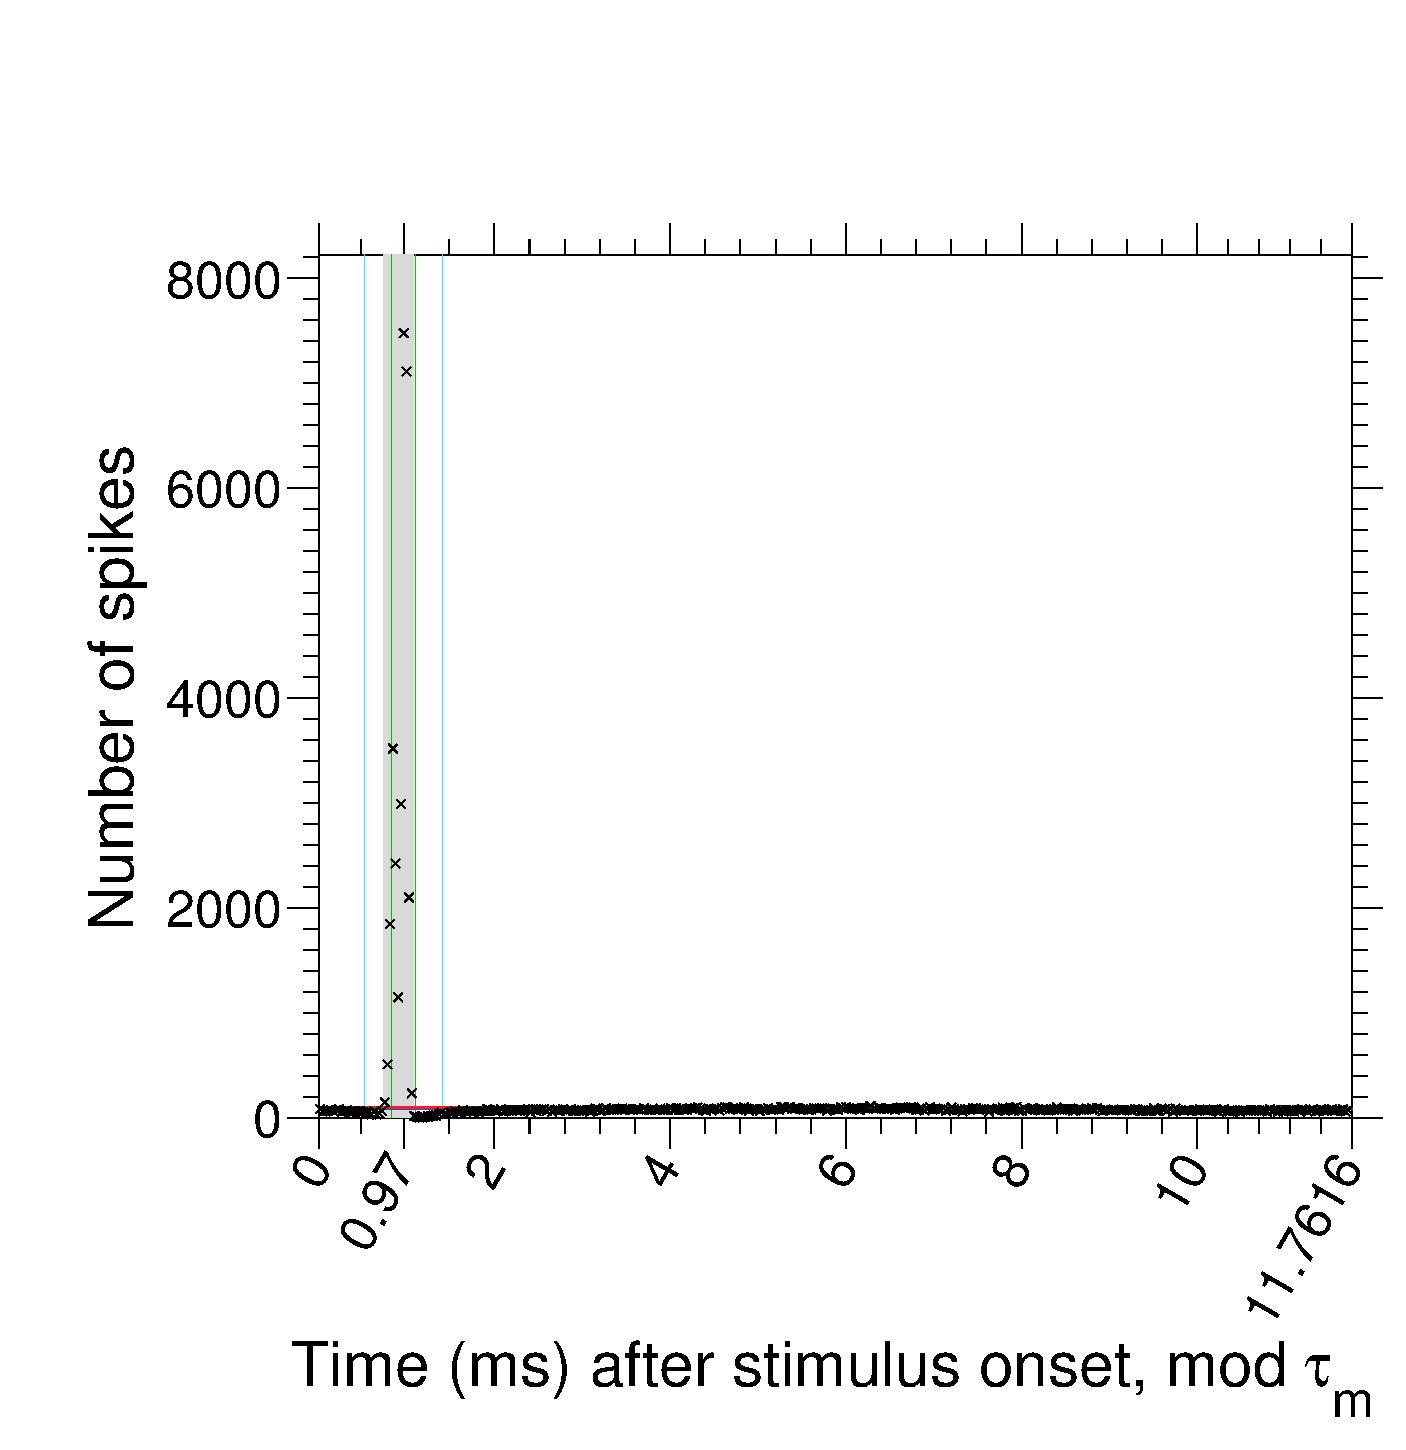
\includegraphics[width=\linewidth]{%
%%figs/info/monitor_hist_blanco_v4_ch4_s336_20120817T085037.eps}
%%    \end{subfigure}
%%    ~~
%%    \begin{subfigure}[b]{0.5\linewidth}
%%        \centering
%%        \caption{}
%%        \label{fig:mahist-j4}
%%        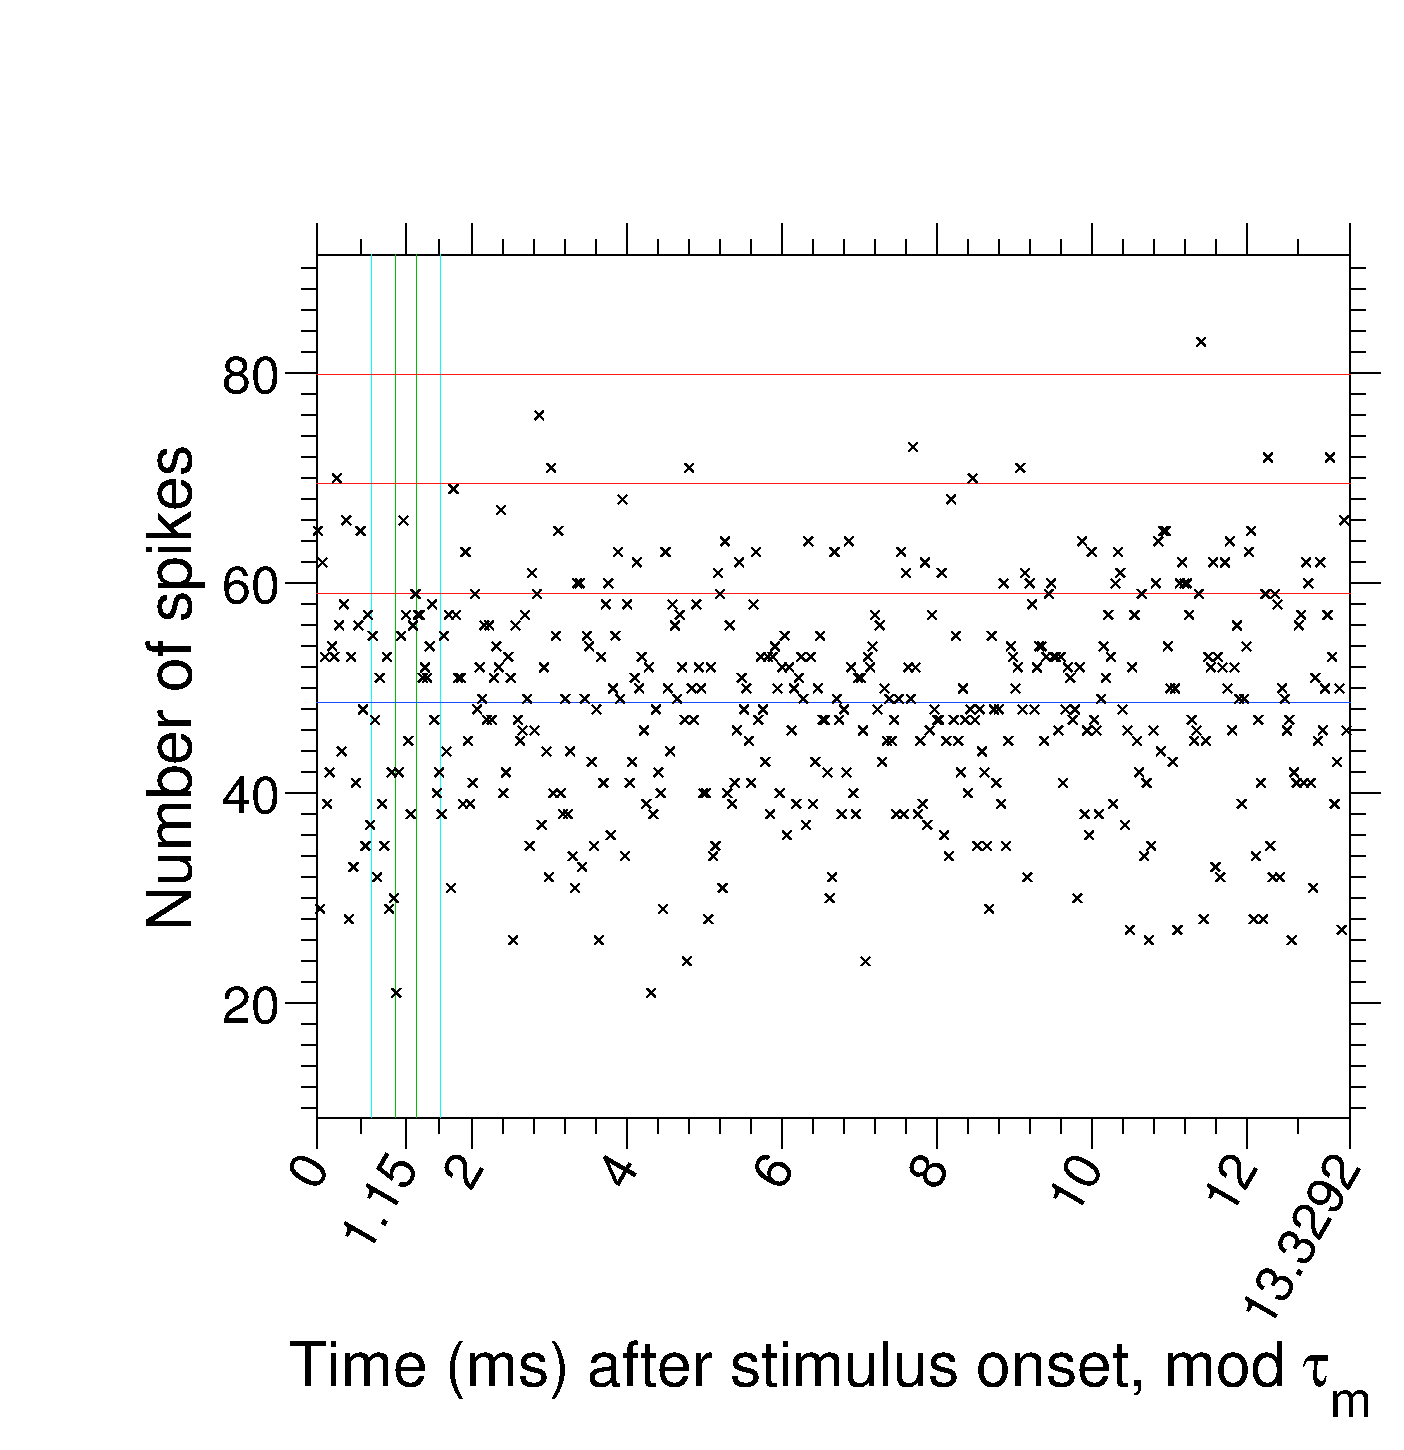
\includegraphics[width=\linewidth]{%
%%figs/info/monitor_hist_jack_v4_ch41_s31_20120817T085111.eps}
%%    \end{subfigure}
%%    \\
%%    \begin{subfigure}[b]{0.5\linewidth}
%%        \centering
%%        \caption{}
%%        \label{fig:mahist-j1s51}
%%        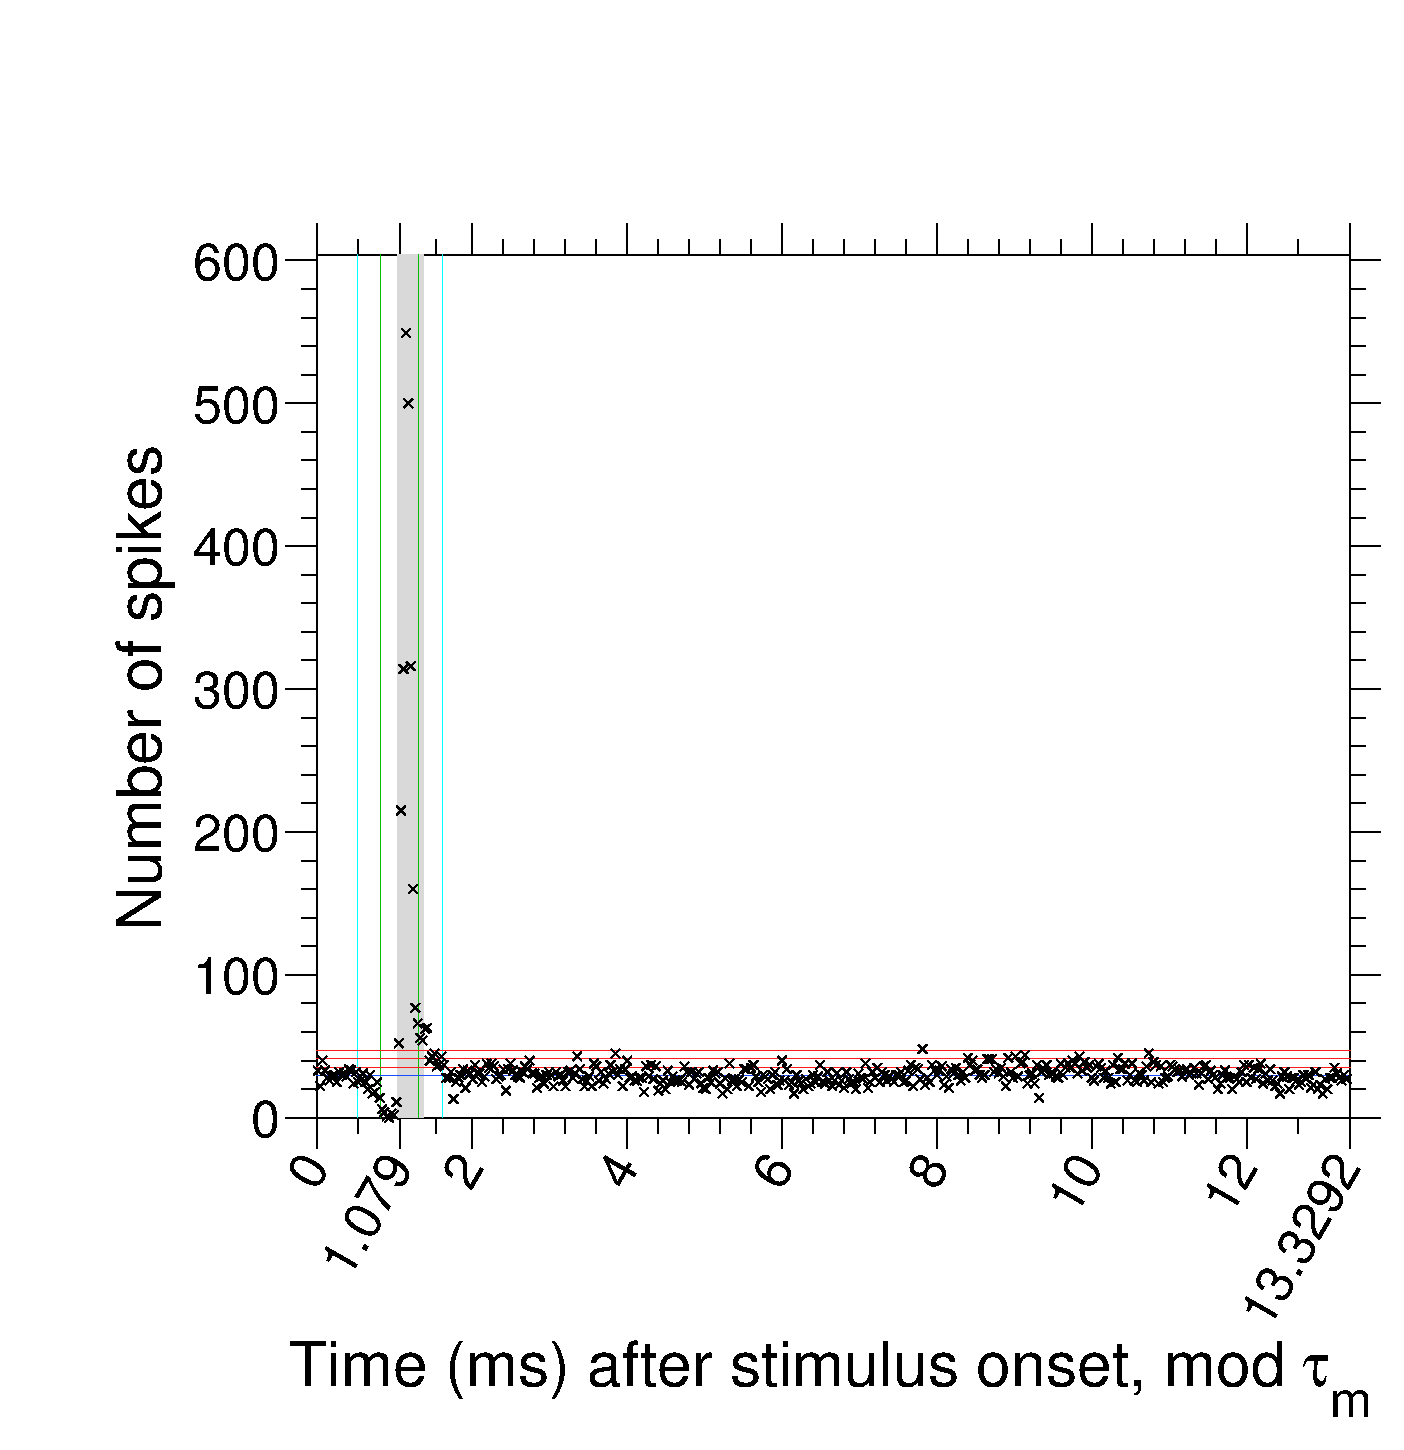
\includegraphics[width=\linewidth]{%
%%figs/info/monitor_hist_jack_v1_ch9_s51_20120817T084845.eps}
%%    \end{subfigure}
%%    ~~
%%    \begin{subfigure}[b]{0.5\linewidth}
%%        \centering
%%        \caption{}
%%        \label{fig:mahist-j1s56}
%%        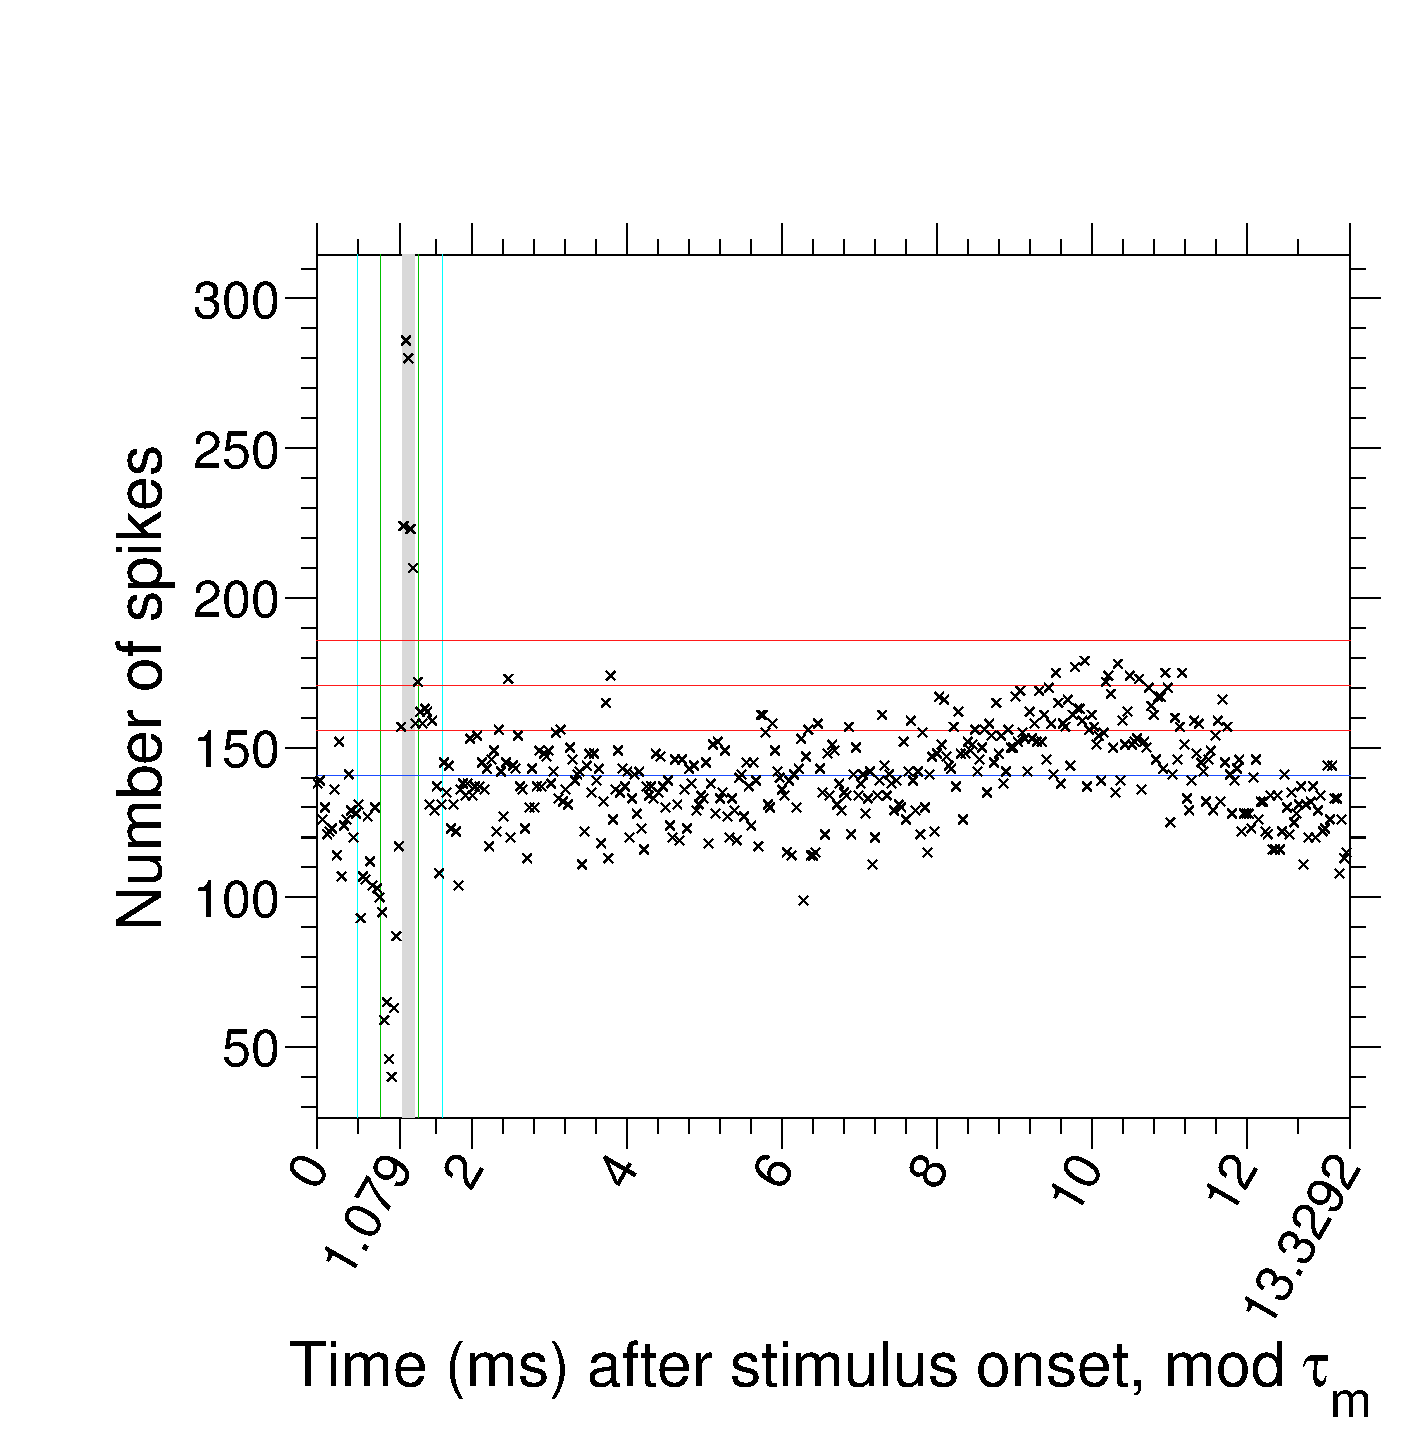
\includegraphics[width=\linewidth]{%
%%figs/info/monitor_hist_jack_v1_ch9_s56_20120817T084855.eps}
%%    \end{subfigure}
%%    \caption{Crosses: Histogram of spikes in bins of width \SI{0.030716}{ms}.
%%\ref{fig:mahist-b4}: \ac{M1} \ac{V4}, channel 4, session 336; a channel and session very strongly exhibiting the monitor artifact.
%%\ref{fig:mahist-j4}: \ac{M2} \ac{V4}, channel 41, session 31; a dataset where the artifact is not present.
%%\ref{fig:mahist-j1s51}: \ac{M2} \ac{V1}, channel 9, session 51; data strongly presenting the monitor artifact.
%%\ref{fig:mahist-j1s56}: \ac{M2} \ac{V1}, channel 9, session 56; data mildly showing the effect of the monitor artifact.
%%Green vertical lines: extremities of search window (contained between the lines).
%%Cyan vertical lines: extremities of mean region.
%%Blue line: mean of the data (excluding area between cyan lines).
%%Red lines: mean plus 1, 2 and 3 standard deviations respectively.
%%Gray background: Spikes marked as contaminated and scheduled for redaction.
%%}
%%    \label{fig:mahist}
%%\end{figure}

% INSERT HIST FIGURE 

As shown in Fig.~\ref{fig:mahist}, the analysis conforms to our expectations.
However, doing the analysis in this more rigorous manner revealed the contamination was more widespread than previously assumed.
The histograms of spike times indicate that more sessions are contaminated than not, and only a couple of channels are completely clean for every session.

For the most part, the timing of the monitor artifact $\bmod \tau_m$ is very reliable and it affects the same 6 or so bins whenever the data is contaminated.
The contaminated part of each monitor cycle is thus restricted to at most \SI{0.2}{ms}, and, assuming this period of time contains both genuine spikes and artificial spikes, if we simply delete all data points with this \SI{0.2}{ms} window, we will lose at most less than \SI{2}{\percent} of the genuine spikes.
This level of data loss is not terribly significant, and justifiable for the gain in reliability of the remaining dataset, particularly for sessions where artificial spikes seem to be more common than genuine ones.

\begin{table}[hbtp]
\caption{Typical time of the peak in number of spikes due to the monitor artifact effect.
The time is given relative to the start of the monitor refresh as given by the stimulus onset times.
Monitor artifacts occur at $t = t^*_m + k \tau_m$, for $k \in \Z$.
For channels recording from \ac{M2} \ac{V1}, the artifact will occur at one of the two stated times throughout a given session, but which of the two varies from channel-to-channel for any individual session, and from session-to-session for any individual channel.
Why this happens is unclear.}
\label{tab:mapeak}
\begin{center}
\begin{tabular}{rlc}
\toprule
Animal  & Region & Time of artifact peak $t^*_m$ $\pm 0.01$ (\si{\milli\second})
\\
\midrule
M1  & V1    & 0.95
\\
        & V4    & 0.97
\\
M2    & V1    & either 0.97 or 1.19
\\
        & V4    & 1.15
\\
\bottomrule
\end{tabular}
\end{center}
\end{table}

% However it is apparent that this method is not great (see jack v1 ch7 s57)

However, it is possible to do better that this and to isolate and remove only the contaminated bins.
As shown in Fig.~\ref{fig:mahist}, the effect of the artifact is greater for some sessions than others and
From observations on the typical width time of the width and peak time (Table.~\ref{tab:mapeak}) of the artifact, along with its periodicity ($\tau_m$), the following method of removal was devised and implemented.
\begin{enumerate}
\item Perform the modulo $\tau_m$ and take the histogram as described above.
\item Define the ``search region'' as bins which contain spike within $t^*_m \pm \SI{0.130}{ms}$, so we have one bin more than the anticipated artifact width in either direction.
      (For \ac{M2} \ac{V1}, we use the range (0.968 - 0.130 , 1.190 + 0.130)\si{\milli\second}.)
\item Find the mean, $\mu$, and standard deviation, $\sigma$, of all the bins which are at least 10 away (\SI{0.3}{ms} away) from the search region.
      We also exclude the final bin since $0.030716 \bmod \tau_m \neq 0$ and it is only part-full.
\item If any one of the bins in the search region exceeds $\mu + 3 \sigma$, we declare the session contaminated and proceed with the following steps.
      If not, it is declared intact and left as it is.
\item All bins in the search region which contain more than $\mu + 3 \sigma$ spikes are declared contaminated.
\item Let $t_m$ denote the time of the centre of the bin in the search region containing the most spikes.
\item All bins which contain spikes within $t_m \pm \SI{0.1}{ms}$ are placed in ``quarantine''.
\item All quarantined bins which contain more than $\mu + 2.5 \sigma$ spikes are declared contaminated.
\item All bins between the first and last contaminated bins are declared contaminated.
\item Consider immediate neighbours of the first bin and if they are also contain more than $\mu + 2.5 \sigma$ spikes, they are declared contaminated.
\item Repeat the above step until either a neighbour is found which is not contaminated, or until a maximum of three bins have been added to the contaminated region.
\item Consider immediate neighbours of the last bin and if they are also contain more than $\mu + 2.5 \sigma$ spikes, they are declared contaminated.
\item Repeat the above step until either a neighbour is found which is not contaminated, or until a maximum of three bins have been added to the contaminated region.
\item Consider the full dataset of spikes for this particular channel and session.
\item For each spike, consider which bin its spike time would be arranged into.
\item If it is a contaminated bin, the spike is removed from the dataset.
\end{enumerate}

This allows us to have prior assumptions about the location and width of the monitor artifact effect, but be flexible about exactly where it falls and which sets of bins are affected.
It is possible that the dynamically targeted removal method may cause issues due to inconsistency in the data across different sessions, but there is a clearly a gain in the amount of preserved data and a gain in the reliability of the data which remains.

%------------------------------------------------------------------------------
\FloatBarrier
\subsection{Session-based analysis}

merged all neurons together for a single channels

Neurolynx NSE files were loaded into MATLAB using the Neurolynx supplied code when operating on Windows, and an version 6 of an unofficial port for Linux (recommended by Neurolynx) otherwise.%
\footnote{Available at
\\ \url{http://www.urut.ch/new/serendipity/index.php?/pages/downloads.html}}

The information was computed for each day of training (hereafter referred to as a session), for each of the channels from which recordings were available.
To gauge the typical behaviour of a neuron, the mean was taken over all the channels.
The mutual information between the spiking activity during test presentation and the identity of the test stimulus was computed
using a spike-timing based code.
This computation was done using the \verb|information| function from the freely available Information Break-down Toolbox \citep{Magri2009} for MATLAB.%
\footnote{Available at \url{http://www.ibtb.org}}

A moving window of $\SI{20}{ms}$ was taken and subdivided into 5 sequential bins, each of $\SI{4}{ms}$.
The number of spikes within each of the 5 bins was totalled up to provide a code letter for the bin.
The combination of the 5 sequential counts forms a codeword.

This is performed across all the trials in a session with the $\SI{20}{ms}$ window placed with the same offset relative to the test stimulus onset.
By assembling the trials according to their test contrast, the mutual information between the contrast and the spiking activity in this window can be computed.

Following the methods employed by the research group, only trials in which the monkey responded correctly were used for this analysis.

%------------------------------------------------------------------------------
% 5bins of 4ms
% figs/info/I_sessionwise_blanco_v1_chmean23_s343-359_oc1_5bins_of_4ms_dr_naive_pcolorhot_20120815T150057.png
% figs/info/I_sessionwise_blanco_v4_chmean31_s307,308,311,313,314,317,318,320,321,329-341_oc1_5bins_of_4ms_dr_naive_pcolorhot_20120815T150100.png
% figs/info/I_sessionwise_jack_v1_chmean25_s51-72_oc1_5bins_of_4ms_dr_naive_pcolorhot_20120815T150049.png
% figs/info/I_sessionwise_jack_v4_chmean20_s24-49_oc1_5bins_of_4ms_dr_naive_pcolorhot_20120815T150053.png
% 1 bin of 20ms
% figs/info/I_sessionwise_blanco_v1_chmean23_s343-359_oc1_1bins_of_20ms_dr_naive_pcolorhot_20120815T190833.png
% figs/info/I_sessionwise_blanco_v4_chmean31_s307,308,311,313,314,317,318,320,321,329-341_oc1_1bins_of_20ms_dr_naive_pcolorhot_20120815T190836.png
% figs/info/I_sessionwise_jack_v1_chmean25_s51-72_oc1_1bins_of_20ms_dr_naive_pcolorhot_20120815T190825.png
% figs/info/I_sessionwise_jack_v4_chmean20_s24-49_oc1_1bins_of_20ms_dr_naive_pcolorhot_20120815T190829.png
% 
% figs/info/I_sessionwise_blanco_v1_chmean23_s343-359_oc1_5bins_of_4ms_dr_naive_pcolorhot_20120815T202102.png
% figs/info/I_sessionwise_blanco_v4_chmean31_s307,308,311,313,314,317,318,320,321,329-341_oc1_5bins_of_4ms_dr_naive_pcolorhot_20120815T202106.png
% figs/info/I_sessionwise_jack_v1_chmean25_s51-72_oc1_5bins_of_4ms_dr_naive_pcolorhot_20120815T202053.png
% figs/info/I_sessionwise_jack_v4_chmean20_s24-49_oc1_5bins_of_4ms_dr_naive_pcolorhot_20120815T202058.png


%%\begin{figure}
%%\centering
%%\subfloat[A big tikz picture.\label{fig:one}]{%
%%  \makebox[\textwidth][l]{% %%% as above
%%  \resizebox{.45\largefigure}{!}{%
%%    \input{fig/tikzfile}}}}%
%%\hfill%
%%\subfloat[Another big tikz picture.\label{fig:two}]{%
%%  \makebox[\textwidth][l]{% %%% as above
%%  \resizebox{.45\largefigure}{!}{%
%%    \input{fig/tikzfile}}}}%
%%\caption{Two tikz pictures}
%%\label{fig:label}
%%\end{figure}
%%
%%\begin{figure}%
%%\centering
%%\subfloat[][]{...figure code...}%
%%\qquad
%%\subfloat[][]{...figure code...}%
%%\caption{Here are the first two figures of a continued figure.}%
%%\label{fig:cont}%
%%\end{figure}

\begin{figure}[htbp]%
    \centering
    \subfloat[][\ac{M1} \ac{V1}.\label{fig:sessb1}]{%
        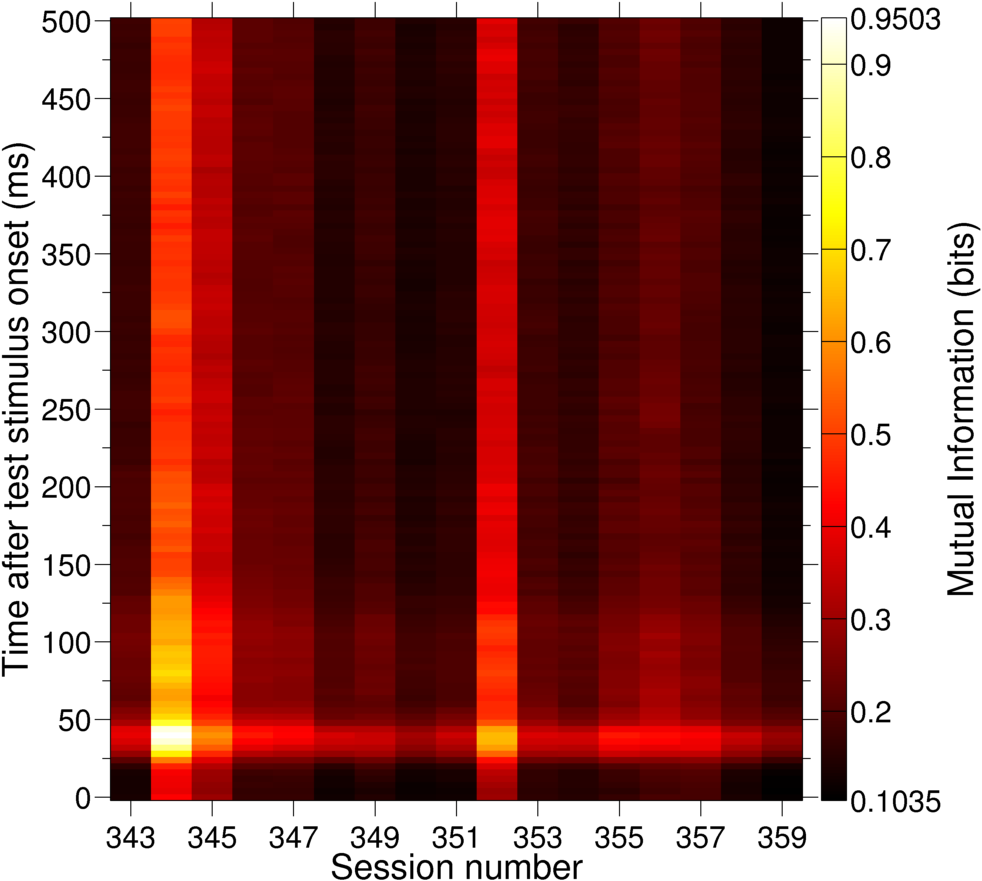
\includegraphics[scale=.25]{%
figs/info/I_sessionwise_blanco_v1_chmean23_s343-359_oc1_5bins_of_4ms_dr_naive_pcolorhot_20120815T202102.png}
    }%
    ~~
    \subfloat[][\ac{M1} \ac{V4}.\label{fig:sessb4}]{%
        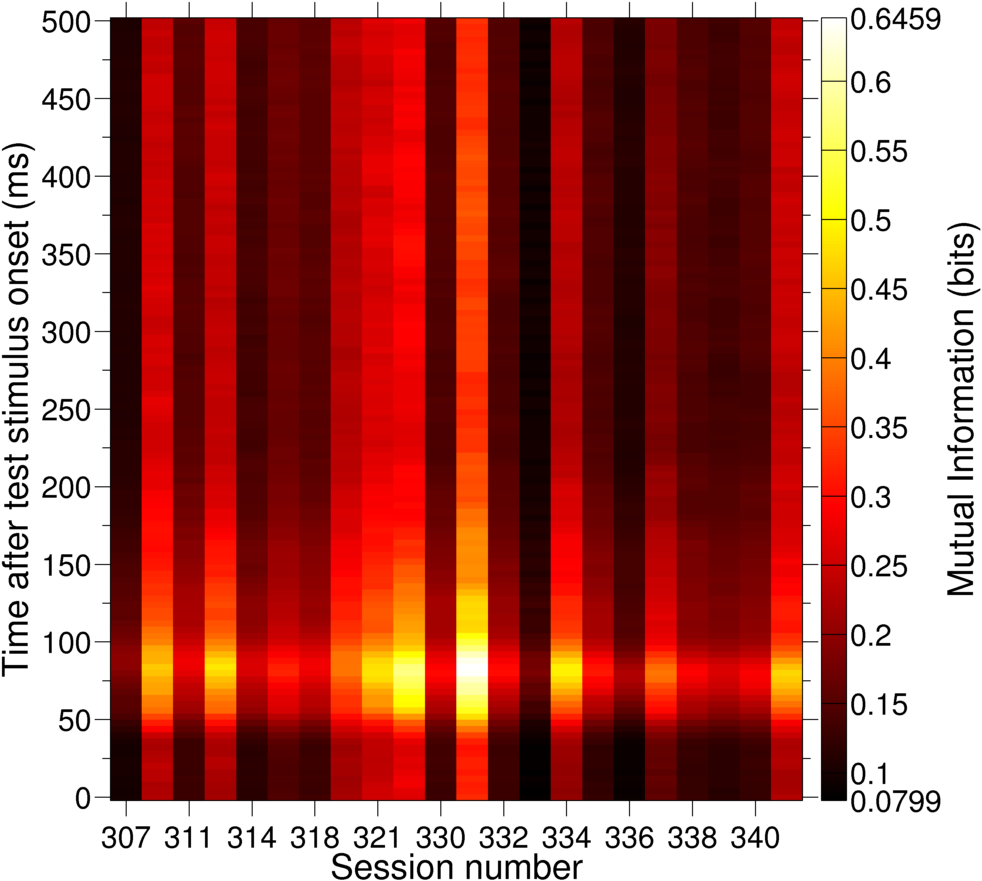
\includegraphics[scale=.25]{%
figs/info/I_sessionwise_blanco_v4_chmean31_s307,308,311,313,314,317,318,320,321,329-341_oc1_5bins_of_4ms_dr_naive_pcolorhot_20120815T202106.png}
    }%
    \\
    \subfloat[][\ac{M2} \ac{V1}.\label{fig:sessj1}]{%
        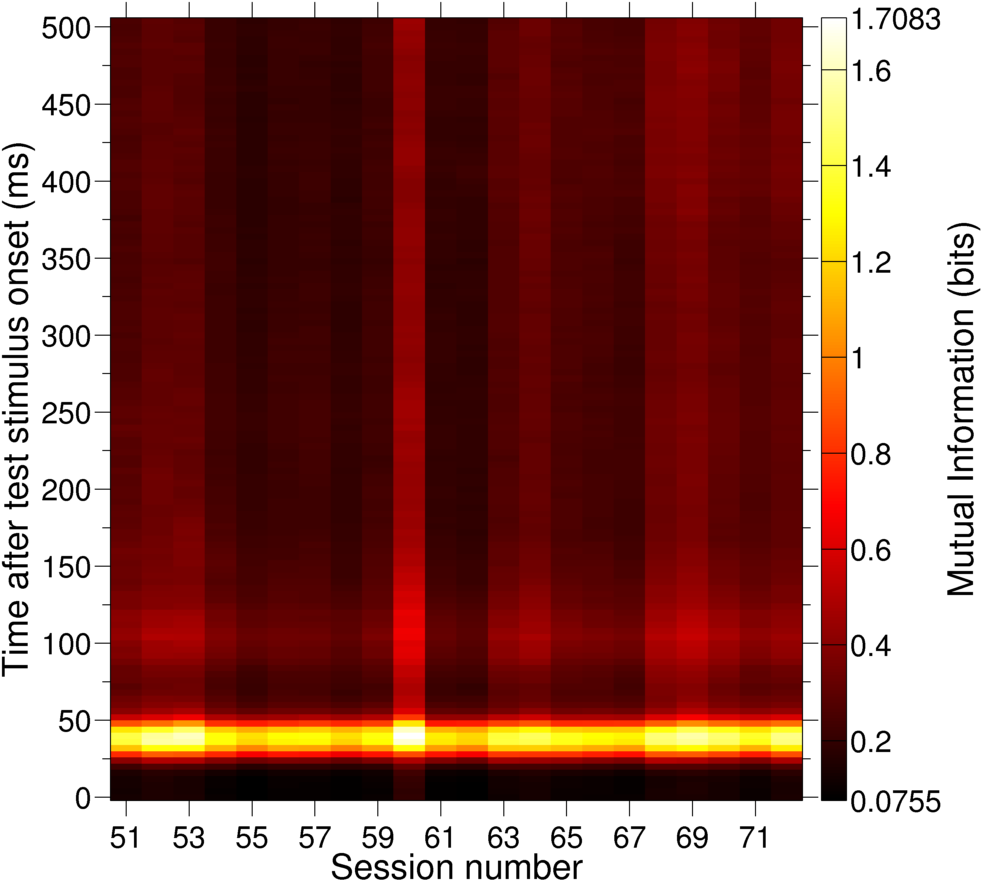
\includegraphics[scale=.25]{%
figs/info/I_sessionwise_jack_v1_chmean25_s51-72_oc1_5bins_of_4ms_dr_naive_pcolorhot_20120815T202053.png}
    }%
    ~~
    \subfloat[][\ac{M2} \ac{V4}.\label{fig:sessj4}]{%
        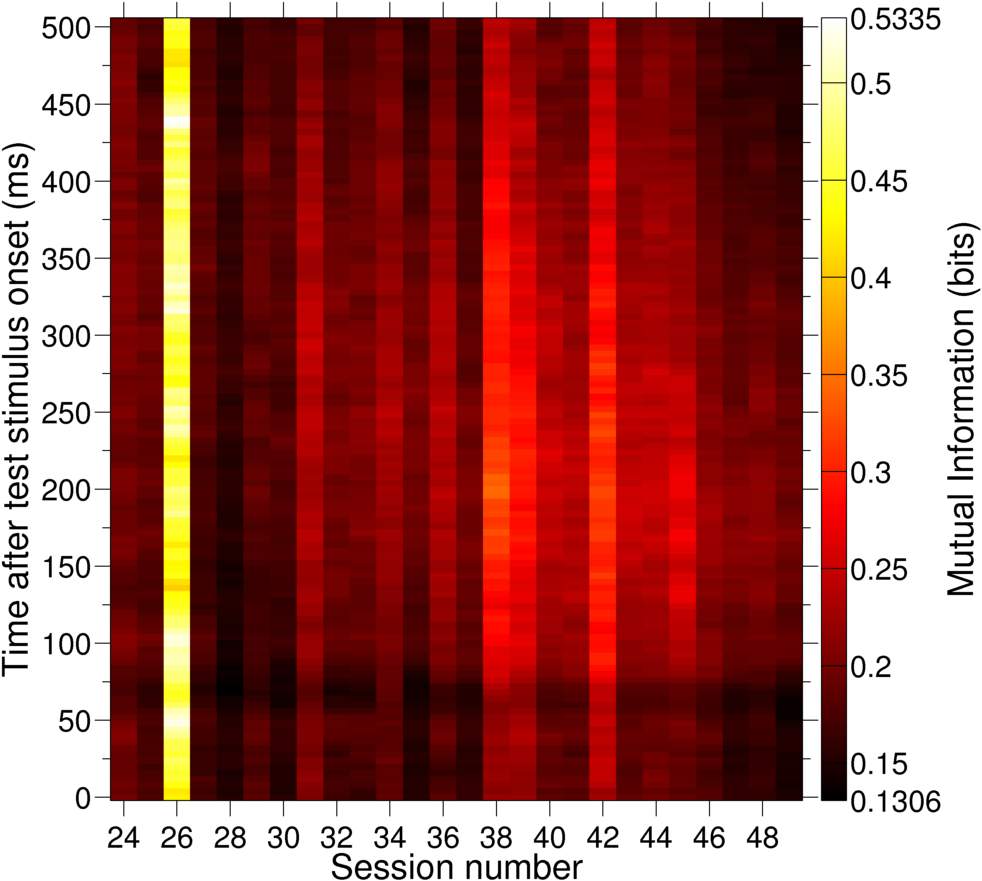
\includegraphics[scale=.25]{%
figs/info/I_sessionwise_jack_v4_chmean20_s24-49_oc1_5bins_of_4ms_dr_naive_pcolorhot_20120815T202058.png}
    }%
    \caption{Mutual information between the test stimulus and the neural activity during test presentation.
The mutual information with the test stimulus is taken for a spike timing based code for a \SI{20}{ms} window of spiking activity, sampled with the start of the window offset ($y$-axis) from \SI{0}{ms} up to \SI{500}{ms} after test stimulus onset (which is slightly more than \SI{20}{ms} before test stimulus offset).
The sampling is in intervals of \SI{5}{ms}, so any 4 adjacent squares within each session are highly correlated.
The recording session number for the data is given along the $x$-axis, and the number of days the animal has been trained for increases from left to right.
Average mutual information across all the channels is denoted by the pseudo-colour of each of the rectangular patches, centred around the $(x,y)$ co-ordinate to which the measurement relates.
In each case the average is taken across all available channel data: \ref{fig:sessb1}~23 channels, \ref{fig:sessb4}~30 channels, \ref{fig:sessj1}~25 channels, \ref{fig:sessj4}~20 channels.
% The \ac{PT} bias correction method was used (see text).
No bias correction method was used.
}
    \label{fig:sess}
\end{figure}

% figs/info/I_sessionwise_blanco_v1_chmean23_s343-359_oc1_5bins_of_4ms_dr_pt_pcolorhot_20120811T130028.eps
% figs/info/I_sessionwise_blanco_v4_chmean31_s307,308,311,313,314,317,318,320,321,329-341_oc1_5bins_of_4ms_dr_pt_pcolorhot_20120811T130522.eps
% figs/info/I_sessionwise_jack_v1_chmean25_s51-72_oc1_5bins_of_4ms_dr_pt_pcolorhot_20120811T130003.eps
% figs/info/I_sessionwise_jack_v4_chmean20_s24-49_oc1_5bins_of_4ms_dr_pt_pcolorhot_20120811T133212.eps

The results of this initial analysis are shown in Fig.~\ref{fig:sess}.
% Although the relationship between different window offsets and the mutual information is similar for each of the sessions, the
No trend in information content with learning can be discerned because the measured mutual information content varies wildly from session-to-session.

% %------------------------------------------------------------------------------
% \chapter{}
% %------------------------------------------------------------------------------
% \subsection{Methods}


% Demonstrate how this is dominated by the number of trials in the session, regardless of bias correction technique

% figs/info/ntrialsIbyNindiv_blanco_v1_dr_naive_20120812T164553.eps
% figs/info/ntrialsIbyNindiv_blanco_v4_dr_naive_20120812T164553.eps
% figs/info/ntrialsIbyNindiv_jack_v1_dr_naive_20120812T164553.eps
% figs/info/ntrialsIbyNindiv_jack_v4_dr_naive_20120812T164553.eps
%
% figs/info/ntrialsIandNindiv_blanco_v1_dr_naive_20120812T175154.eps
% figs/info/ntrialsIandNindiv_blanco_v4_dr_naive_20120812T175154.eps
% figs/info/ntrialsIandNindiv_jack_v1_dr_naive_20120812T175154.eps
% figs/info/ntrialsIandNindiv_jack_v4_dr_naive_20120812T175154.eps
%
% figs/info/ntrialsIandNindiv_blanco_v1_dr_naive_1bins_of_20ms_20120815T200333.eps
% figs/info/ntrialsIandNindiv_blanco_v4_dr_naive_1bins_of_20ms_20120815T200333.eps
% figs/info/ntrialsIandNindiv_jack_v1_dr_naive_1bins_of_20ms_20120815T200333.eps
% figs/info/ntrialsIandNindiv_jack_v4_dr_naive_1bins_of_20ms_20120815T200333.eps
% 
% figs/info/ntrialsIandNindiv_blanco_v1_dr_naive_5bins_of_4ms_20120815T201856.eps
% figs/info/ntrialsIandNindiv_blanco_v4_dr_naive_5bins_of_4ms_20120815T201856.eps
% figs/info/ntrialsIandNindiv_jack_v1_dr_naive_5bins_of_4ms_20120815T201856.eps
% figs/info/ntrialsIandNindiv_jack_v4_dr_naive_5bins_of_4ms_20120815T201856.eps
% 
% % \begin{figure}[htbp]
% %     \begin{subfigure}[b]{0.5\linewidth}
% %         \centering
% %         \caption{\ac{M1} \ac{V1}}
% %         \label{fig:IandNb1}
% %         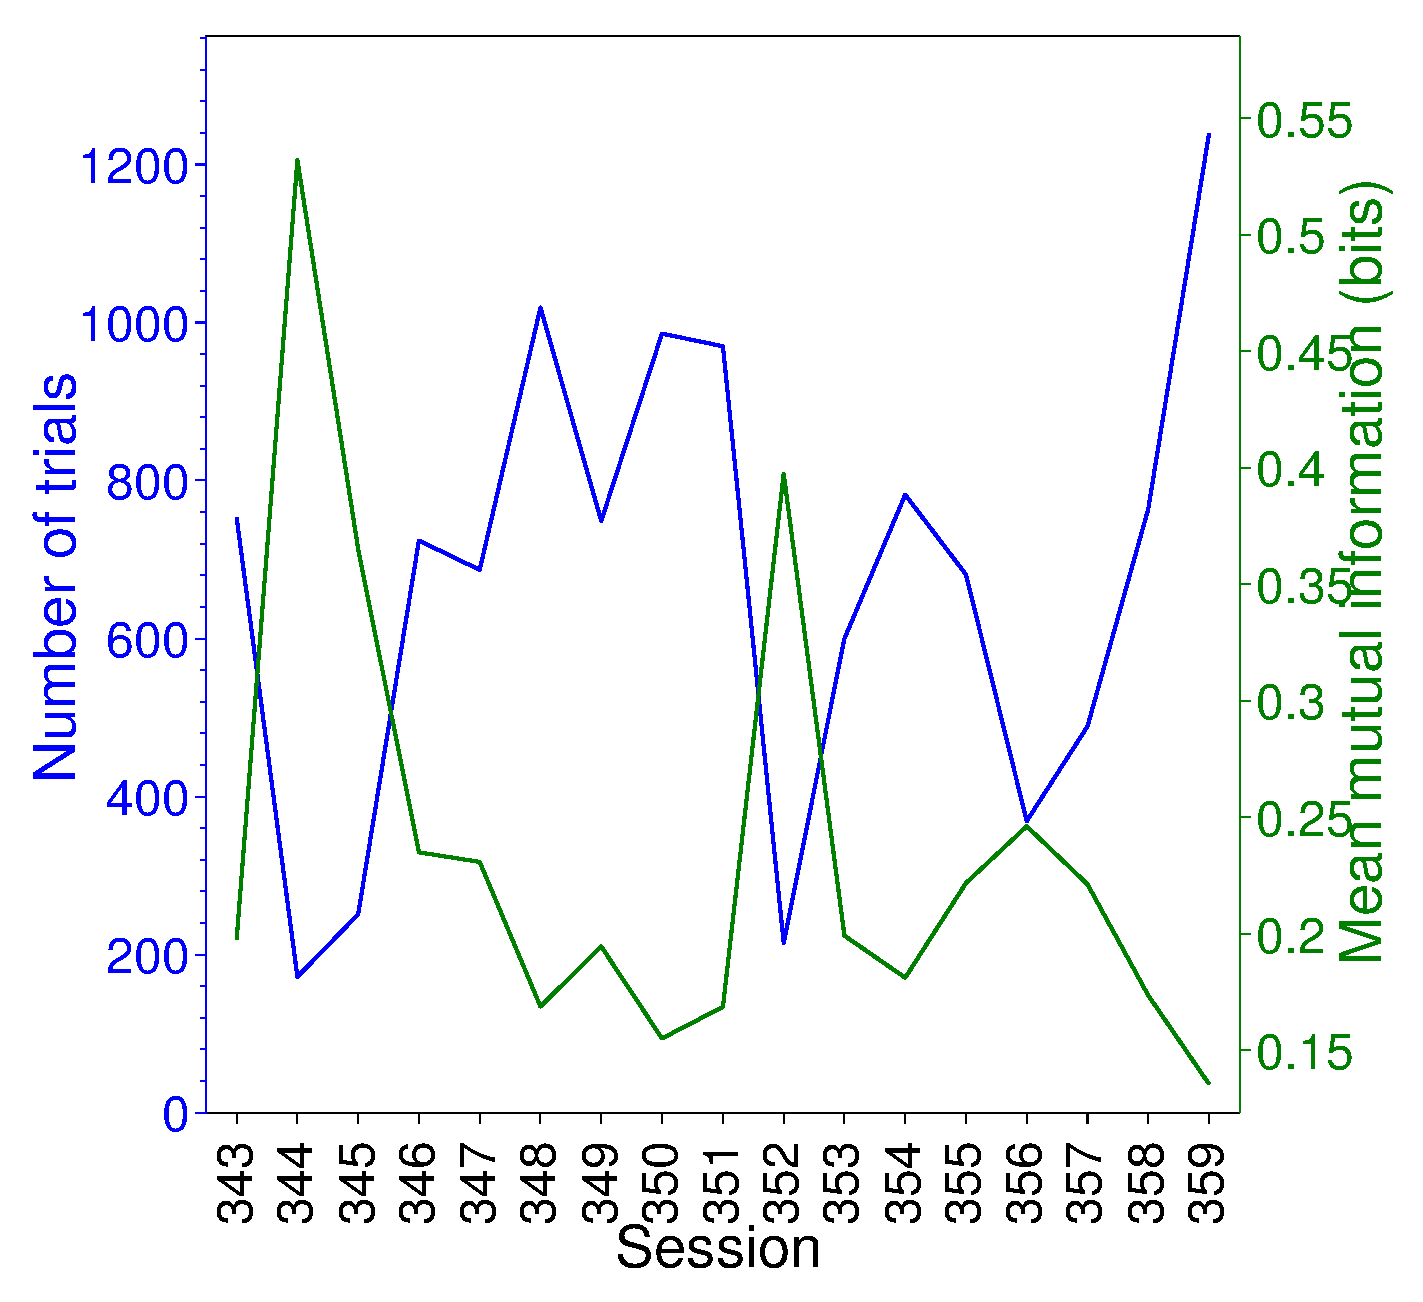
\includegraphics[width=\linewidth]{%
% % figs/info/ntrialsIandNindiv_blanco_v1_dr_naive_5bins_of_4ms_20120815T201856.eps}
% %     \end{subfigure}
% %     \begin{subfigure}[b]{0.5\linewidth}
% %         \centering
% %         \caption{\ac{M1} \ac{V4}}
% %         \label{fig:IandNb4}
% %         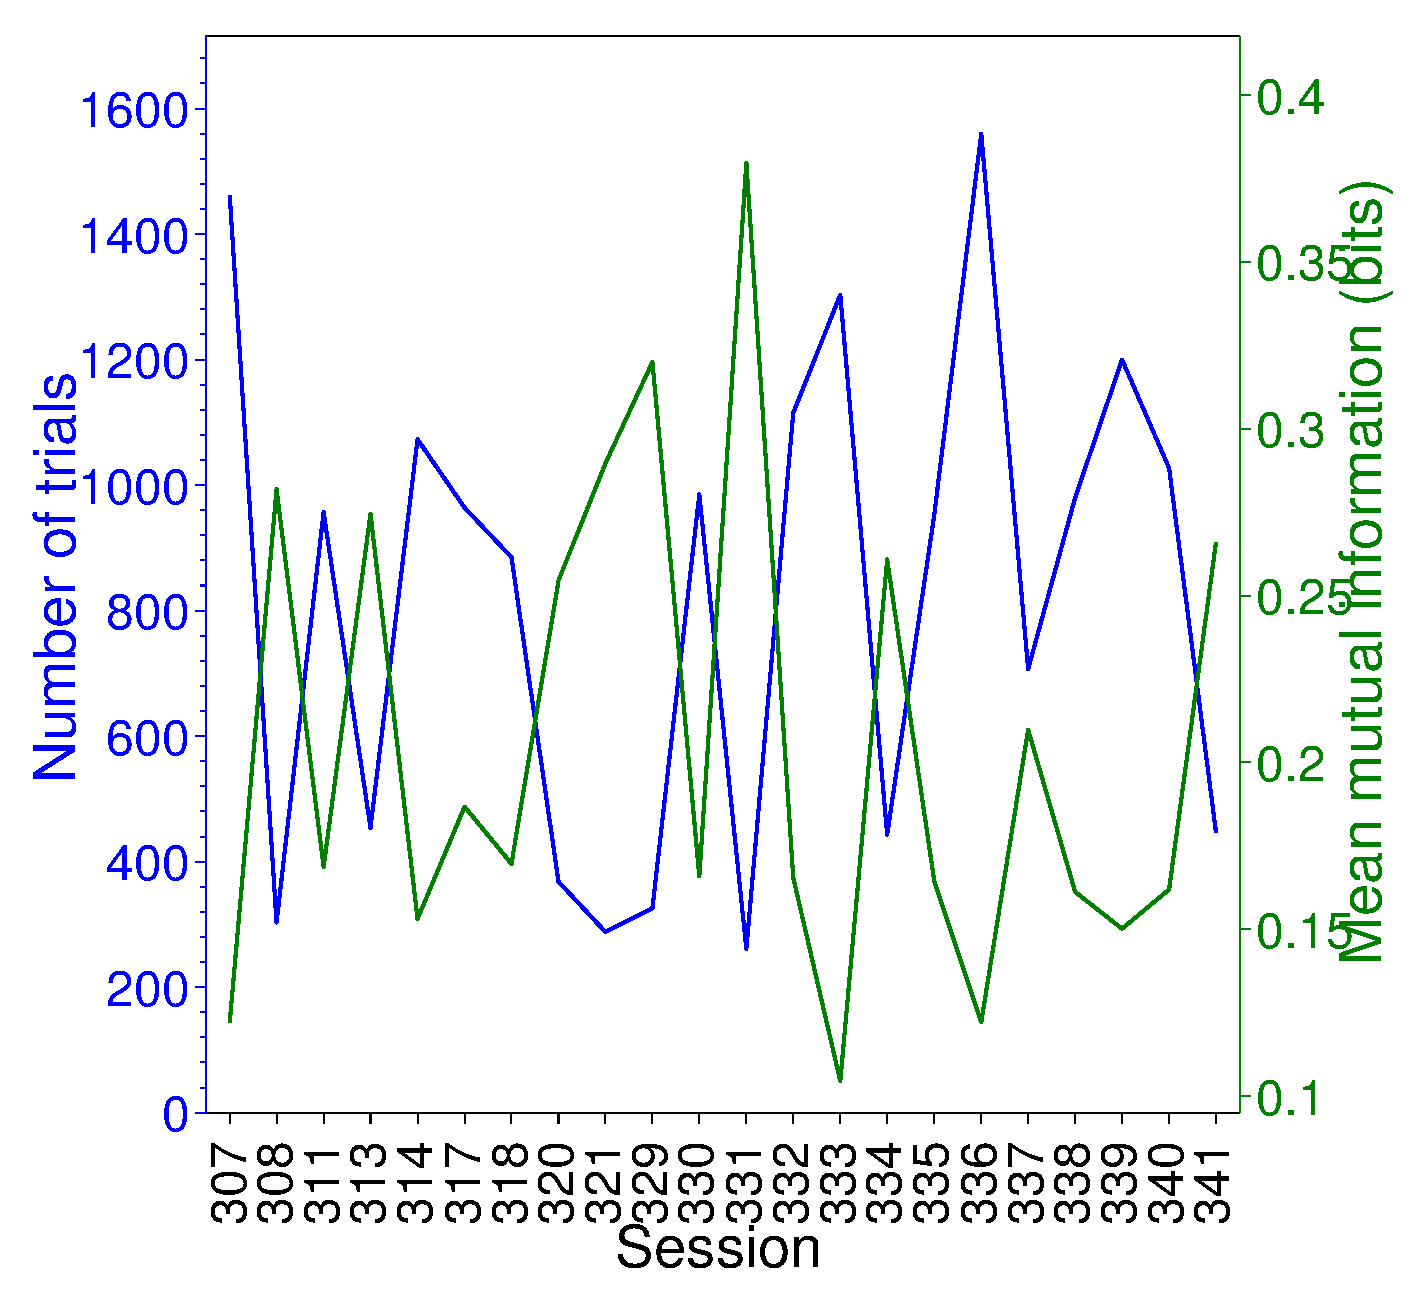
\includegraphics[width=\linewidth]{%
% % figs/info/ntrialsIandNindiv_blanco_v4_dr_naive_5bins_of_4ms_20120815T201856.eps}
% %     \end{subfigure}
% %     \\
% %     \begin{subfigure}[b]{0.5\linewidth}
% %         \centering
% %         \caption{\ac{M2} \ac{V1}}
% %         \label{fig:IandNj1}
% %         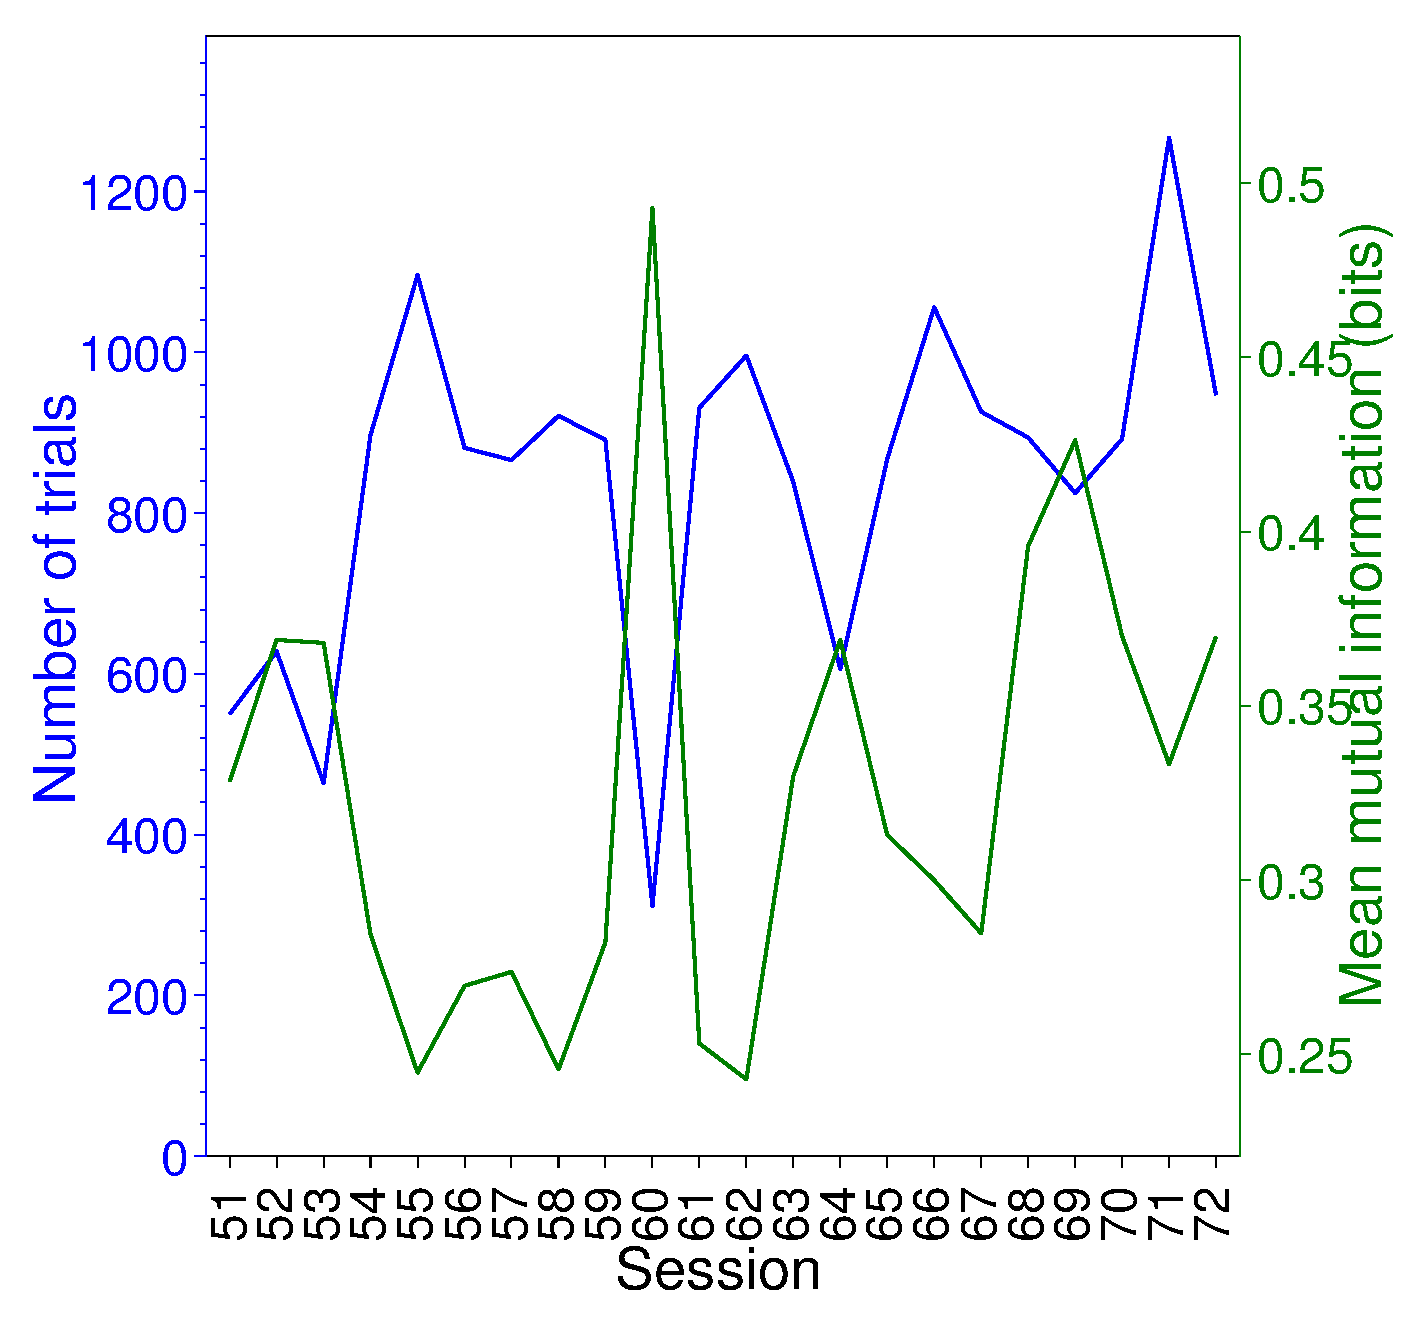
\includegraphics[width=\linewidth]{%
% % figs/info/ntrialsIandNindiv_jack_v1_dr_naive_5bins_of_4ms_20120815T201856.eps}
% %     \end{subfigure}
% %     \begin{subfigure}[b]{0.5\linewidth}
% %         \centering
% %         \caption{\ac{M2} \ac{V4}}
% %         \label{fig:IandNj4}
% %         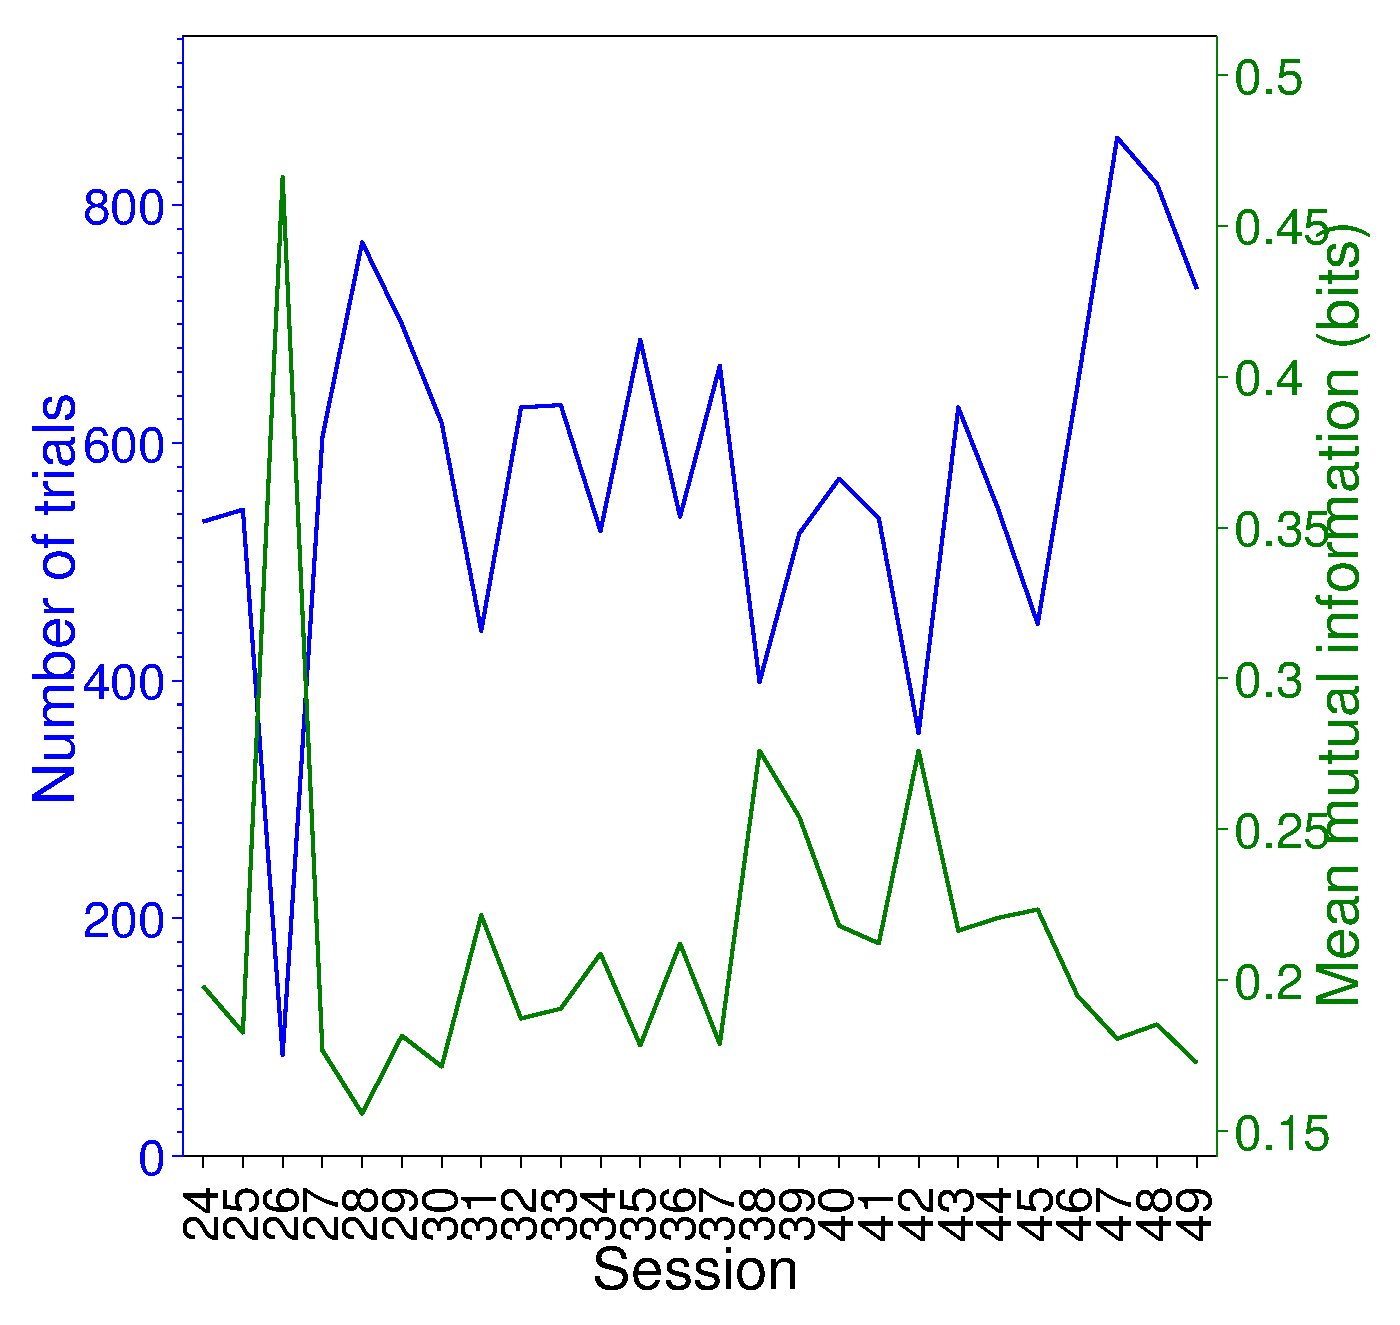
\includegraphics[width=\linewidth]{%
% % figs/info/ntrialsIandNindiv_jack_v4_dr_naive_5bins_of_4ms_20120815T201856.eps}
% %     \end{subfigure}
% %     \caption{Mutual information seems to be anti-correlated with the number of trials in the session. The number of correctly responded trials in each session is plotted on top of the mean information in individual sessions. The mutual information was not corrected for bias, and averaged across the whole period of test stimulus presentation.
% % %There is a missing data point for \ac{M2} \ac{V4} because in one session there were not enough trials per condition for the \ac{QE} algorithm to function.
% % }
% %     \label{fig:IandN}
% % \end{figure}

Fig.~\ref{fig:IandN} shows that the changes in the measured mutual information are dominated by the number of trials in the session, not by increases with perceptual learning (corresponding to increments in the session number).
The only exception to this rule seems to be for \ac{M2} \ac{V1}, shown in Fig.~\ref{fig:IandNj1}, where the information increases with learning despite an increase in the number of trials per session over this period.

% figs/info/ntrialsIvsinvNcombindiv_blanco_v1_20120812T164553.eps
% figs/info/ntrialsIvsinvNcombindiv_blanco_v4_20120812T164553.eps
% figs/info/ntrialsIvsinvNcombindiv_jack_v1_20120812T164553.eps
% figs/info/ntrialsIvsinvNcombindiv_jack_v4_20120812T164553.eps
% 
% figs/info/ntrialsIvsinvNcombindiv_blanco_v1_5bins_of_4ms_20120815T204808.eps
% figs/info/ntrialsIvsinvNcombindiv_blanco_v4_5bins_of_4ms_20120815T204808.eps
% figs/info/ntrialsIvsinvNcombindiv_jack_v1_5bins_of_4ms_20120815T204808.eps
% figs/info/ntrialsIvsinvNcombindiv_jack_v4_5bins_of_4ms_20120815T204808.eps
% 
% % \begin{figure}[htbp]
% %     \begin{subfigure}[b]{0.5\linewidth}
% %         \centering
% %         \caption{\ac{M1} \ac{V1}}
% %         \label{fig:IvNb1}
% %         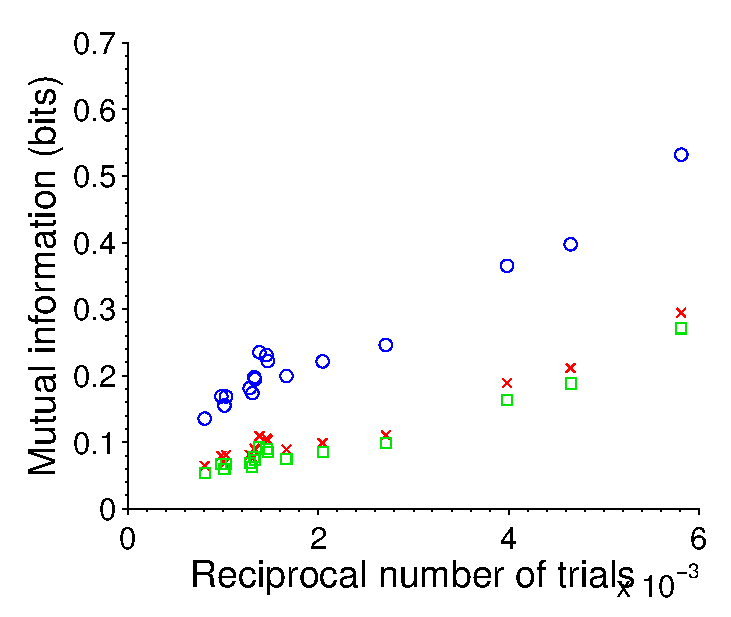
\includegraphics[width=\linewidth]{%
% % figs/info/ntrialsIvsinvNcombindiv_blanco_v1_5bins_of_4ms_20120815T204808.eps}
% %     \end{subfigure}
% %     \begin{subfigure}[b]{0.5\linewidth}
% %         \centering
% %         \caption{\ac{M1} \ac{V4}}
% %         \label{fig:IvNb4}
% %         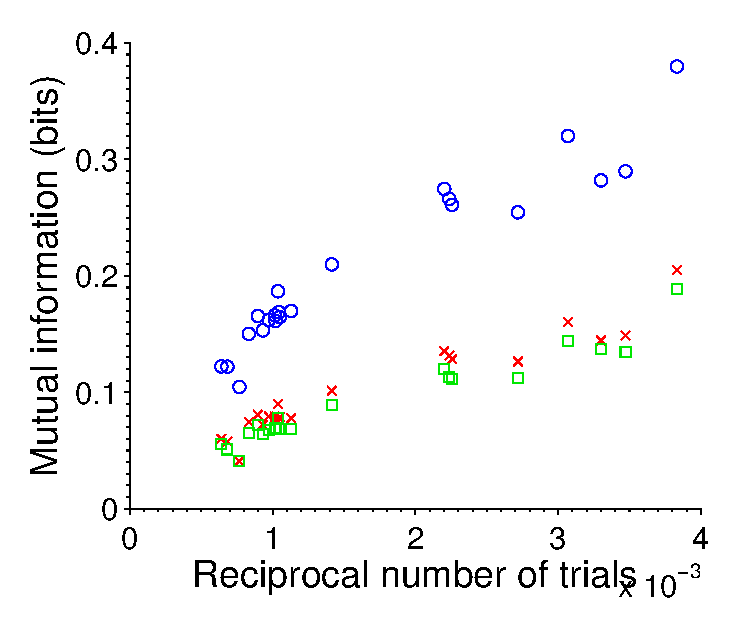
\includegraphics[width=\linewidth]{%
% % figs/info/ntrialsIvsinvNcombindiv_blanco_v4_5bins_of_4ms_20120815T204808.eps}
% %     \end{subfigure}
% %     \\
% %     \begin{subfigure}[b]{0.5\linewidth}
% %         \centering
% %         \caption{\ac{M2} \ac{V1}}
% %         \label{fig:IvNj1}
% %         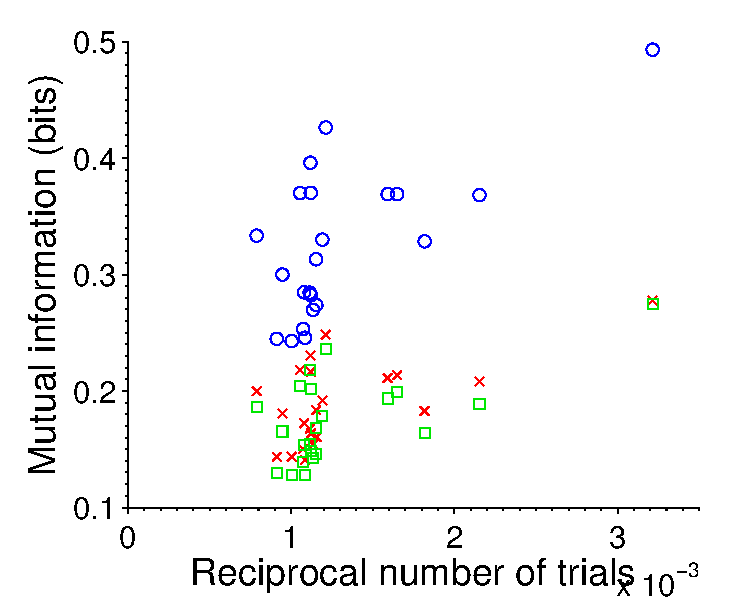
\includegraphics[width=\linewidth]{%
% % figs/info/ntrialsIvsinvNcombindiv_jack_v1_5bins_of_4ms_20120815T204808.eps}
% %     \end{subfigure}
% %     \begin{subfigure}[b]{0.5\linewidth}
% %         \centering
% %         \caption{\ac{M2} \ac{V4}}
% %         \label{fig:IvNj4}
% %         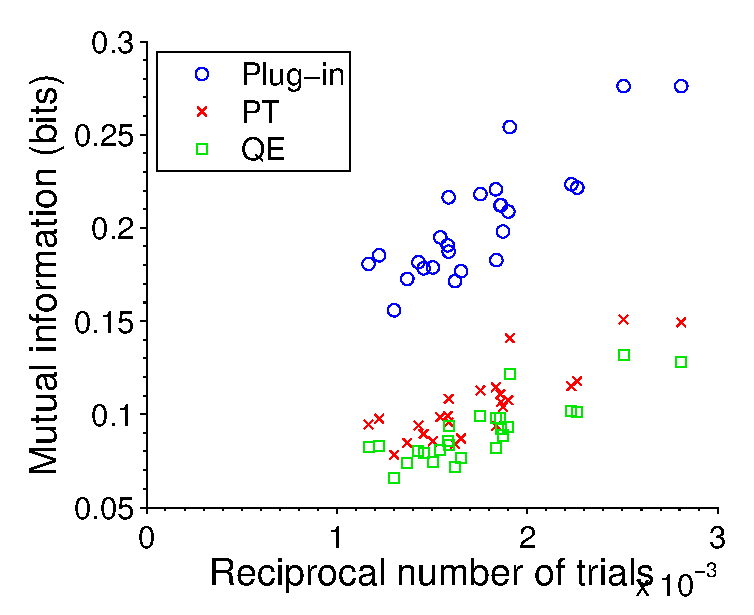
\includegraphics[width=\linewidth]{%
% % figs/info/ntrialsIvsinvNcombindiv_jack_v4_5bins_of_4ms_20120815T204808.eps}
% %     \end{subfigure}
% %     \caption{Mutual information is inversely correlated with the number of trials in the session. The mutual information for a single session is averaged over all channels, and averaged over all times during stimulus presentation, and plotted against the reciprocal of the number of trials in the session ($\nicefrac{1}{N}$). Plug-in:~without bias correction. \ac{PT}:~using the Panzeri-Treves method to correct for bias \citep{Panzeri1996}. \ac{QE}:~using quadratic extrapolation for bias correction \citep{Strong1998}.
% % %There is a missing data point for \ac{M2} \ac{V4} because in one session there were not enough trials per condition for the \ac{QE} algorithm to function.
% % }
% %     \label{fig:IvN}
% % \end{figure}

In particular, the measured value for the mutual information is strongly correlated with the reciprocal of the number of trials in the session (Fig.~\ref{fig:IvN}).
The correlation is still very strong even if we use one of the two bias correction techniques.
As discussed above, for \ac{M2} \ac{V1} the number of trials per session and the measured information  are both correlated with time, which reduces the correlation observed in Fig.~\ref{fig:IvNj1}.

The problem is that although \ac{PT} and \ac{QE} both do a reasonable attempt at removing the bias, they are not perfect and some bias will remain.
As the bias is dependent on the number of trials, it is unsurprising the remaining bias follows the same dependency.
In particular, in the asymptotic regime the leading term in the expansion of $I_{\text{measured}}$ is known to be proportional \citep{Treves1995} to $\nicefrac{1}{N}$; the same relationship observed here.

In particular, the difficult faced is changes due to perceptual learning which are of interest may only be slight, but the the number of trials per session varies five-fold: from 250 up to 1250.
Consequently it is unsurprising that the observed differences in information day-to-day are dominated by the number of trials.

% %------------------------------------------------------------------------------
% \subsection{Results}
% 
% %------------------------------------------------------------------------------
% \chapter{Information Theoretic Analysis (trial-wise)}
% %------------------------------------------------------------------------------

%------------------------------------------------------------------------------
\FloatBarrier
\subsection{Trial-based analysis}

To counter the correlation between measured information and number of trials, an obvious solution is to use the same number of trials for every computation.
We now consider how many trials should be taken at once to obtain a reasonably reliable estimate.

Some rules-of-thumb for the number of trials are offered by \citep{Panzeri2007}.
Let $\overline{R}$ denote the number of possible response codes.
Then, for the bias-uncorrected estimate of mutual information, we need to have at least $N_S \ge 2^{32} \, \overline{R}$ trials per stimulus,
whilst if the \ac{PT} or \ac{QE} bias correction methods are applied, we only need $N_S > 2 \, \overline{R}$.

% The spike detection software was set to only detect spikes at least \SI{3}{ms} apart, and moreover, 
The probability of having two spikes within \SI{4}{ms} from a non-bursting neuron is very low.
For example, a neuron with a high firing rate might fire at \SI{100}{Hz}, which means inter-spike intervals are typically around \SI{10}{ms} (and \SI{100}{Hz} is a high firing rate for the channels in our dataset).
Consequently any \SI{4}{ms} bin will realistically contain either 0 or 1 spikes, and the number of possible response codes in our spike timing code analysis with 5 bins each of \SI{4}{ms} is $\overline{R} = 2^5 = 32$.
In comparison for a spike count code, if we assume spikes cannot be closer together than \SI{3}{ms}, there are between 0 and 7 spikes in any \SI{20}{ms} interval.
Consequently there are $\overline{R} = 8$ possible response codes.

As we wish our analysis to work for both spike timing and spike count codes, using the above rules we need to use at least 64 trials per stimulus to get a reasonable estimate of the information with one of the bias correction methods in place.
Since there are 14 different stimuli, this means at least 896 trials in total are needed.
This presents a dilemma, since most of the sessions are shorter than this, even when both correctly and incorrectly responded trials are included.
Excluding sessions with fewer than 896 trials would severely limit the size of the dataset.
% and the patchwork of holes which would result would limit how much can be read into the results due to  which would result.

The solution found was to concatenate the sessions together and analyse groups of $N$ trials taken from multiple consecutive sessions.
The na\"{i}ve justification for this approach is a ``first-order approximation'' to perceptual learning would be that the monkey gets better at recognising the stimuli every-time they perceive it, and so the most important quantifier for the amount of perceptual learning which has taken place is the total number of trials the monkey has performed to date.

This rather basic assumption neglects several factors which influence the animal's performance, such as their mood during the particular training day; and factors which influence the animal's willingness to work (in turn influencing performance), which depends on their recent level of access to water (the reward used in the study).
For instance, the animal performs less well on Mondays, which follows on from readily available water during the weekend.
Furthermore, the consolidation which occurs during sleep is commonly believed to be important to perceptual learning, and (as this only occurs between training sessions) this effect is completely ignored by this approach.

However, the session-concatenation approach was attempted regardless, and a value of $N_S = 100$ trials per stimulus was chosen.
Though there are enough trials available to use more and reduce the bias further, it is undesirable data from so many sessions at once.

As mentioned in Chap.~\ref{ch:exp}, a delayed repeat is used for any trials to which the animal does not correctly respond.
Consequently, more difficult test stimuli (with contrasts close to the sample contrast) are presented significantly more frequently than easier stimuli.
For instance, when presented with the most difficult test stimuli, the animal will have a success rate only just above \SI{50}{\percent} on the first day of the experiment, rising to around \SI{70}{\percent} by the last day.
For the easiest stimuli, the success rate will be nearly \SI{100}{\percent} throughout.

Say we arrange all the trials into groups based on their stimulus, then take 100 subsequent trials from each of the groups to perform the analysis on.
Due to the different number of trials per stimulus, it will not be long before the trials selected for each stimulus are from very different points in time and from different sessions.\footnote{Even if we only analyse the correctly responded trials, there is still a difference in the number of trials per stimulus due to a limit on the number of repeats of any test condition.
The difference was negligible for \ac{M1}, but accumulated to a 100 trial difference over all the sessions between the most and least correctly responded conditions for \ac{M2}.}
To ensure all the trials are from when the animal has had the same amount of training, we can instead take a group of $S \cdot N_S = 14 \cdot 100 = 1400$ consecutive trials regardless of the stimulus presented and analysed.
The differences in number of trials per stimulus are not particularly important, so long as there are always  enough.

All trials where the monkey completed the trial and gave a response (either correct or incorrect) were included in the analysis.
Trials where the monkey did not complete the task by fixating and then providing a response as required were excluded.
Using both the correct and incorrectly responded trials means our distribution for $P(s)$ is the same as that presented to the monkey, and there are notably more trials available to perform the analysis on.

% Using 50 and 100 trials explored: not considerable difference between results. 100 shown for conciseness

%------------------------------------------------------------------------------
\FloatBarrier
\subsection{Information in fine vs. coarse distinctions}

The difference between information about fine differences in contrast can be studied by only considering trials where the contrast presented is one of the middle 6 contrasts:
\SIlist{22;25;28;32;35;40}{\percent} for \ac{V1} and
\SIlist{27;28;29;31;32;33}{\percent} for \ac{V4}.
To keep the dimensionality of the stimulus the same, this has been compared to the information across some more separated contrasts:
\SIlist{5;15;22;40;50;90}{\percent} for \ac{V1} and
\SIlist{10;15;20;40;50;60}{\percent} for \ac{V4}.
For \ac{V4}, the group of coarsely differentiated contrasts is the outer most six contrasts, but for \ac{V1} the coarsely differentiated contrasts are alternate

%------------------------------------------------------------------------------
\FloatBarrier
\subsection{Information in spike timing code vs. spike count code}

Because the possible responses in the spike timing and count codes have different dimensionality, they have different biases \citep{Panzeri2007} and it is not possible to compare them directly.
Consequently, to investigate how much more information there is in a spike timing based code we must consider a set of responses which have the same dimensionality, but lack the timing information.

To do this, the spike-timing response codes are taken, then shuffled across the 5 bins for every individual trial.%
\footnote{The shuffling of bins was performed using the open source Shuffle.m
available from \url{http://www.mathworks.com/matlabcentral/fileexchange/27076-shuffle}.}
Since the 5 bins are now in a random order, any information contained in their order is lost.
To make ensure the estimate of the information in the spike-timing code with the timing information destroyed was reasonable, the information was measured for five different shuffles%
% \footnote{The five shuffles were performed with a random seed linked to microsecond of execution time.}
 and then the mean was taken.

The information contained in the \SI{4}{ms} level spike timing can then be found by subtracting the mean shuffled information from the unshuffled information.

%------------------------------------------------------------------------------
\FloatBarrier
\subsection{Spontaneous activity}

To check whether changes in the data quality between sessions and other differences between sessions could be influencing the results, the information theoretic analysis was also applied the spontaneous activity from the animal.
In particular, the spontaneous activity from prior to the sample presentation was used, so the animal had not yet seen the test contrast.
Although monkey's brain activity cannot possibly contain any genuine information about the test contrast, we expect to measure a non-zero value for the information content due to the sampling bias.

%------------------------------------------------------------------------------
\subsection{Linear Decoder}
\label{sec:dec-meth-lin}

The input data to the decoding algorithm was chosen to be the total spike count during stimulus presentation from each trial.
This total is taken only for channels known to offer a consistent firing rate across sessions after the spontaneous activity matching process.
If there are 20 such channels in the dataset, taking the total number of spikes during stimulus presentation for each of the channels results in a 20-dimensional vector of population activity on each trial.

It should be noted that using all the spikes during the stimulus presentation period is likely to be sub-optimal, as not necessarily all of this period of time is carrying useful information about the stimuli.
The amount of spikes before the onset response, for instance, is clearly not stimulus dependent as it precedes the neural response to the stimulus, so it will only be a source of noise and  not useful for the decoding.
Furthermore, it is possible that the firing rate during the onset response might be more informative than the average firing rate across the whole presentation period.
However, finding the optimal window from which to take the spikes is an exercise in of itself.

The decoder used was a Fisher linear discriminant classifier.
Given a training dataset of labelled data points in 20D, the classifier will find the optimal 19D hyperplane such that it separates the two classes of points optimally, under the assumption that the two clusters to be separated are multivariate normal distributions.
The vector normal to the hyperplane is 
\begin{equation}
\vec{w} = \Sigma^{-1}\left(\vec{\mu_1}-\vec{\mu_0}\right)
\end{equation}
where $\Sigma$ is the covariance matrix between the two populations, as determined from the available labelled data, and $\vec{\mu_0}$ and $\vec{\mu_1}$ are the computed means of the two distributions.

Once a classifying hyperplane has been found, test data points can be classified by observing the side of the hyperplane on which they fall.
For a new data point, $\vec{x}$,  if
\begin{equation}
\vec{w}\cdot\vec{x}>c
\end{equation}
then we classify $\vec{x}$ as group 1 (higher than \SI{30}{\percent} contrast), otherwise we classify it as 0 (lower).

This was performed using the function \texttt{classify} with type `linear' in MATLAB.
For training and testing of the decoder, leave-one-out classification was used across each session individually.
This means that for a session of 500 trials, the decoder is trained on 499 trials with the spike counts for all the trials and the correct response (higher or lower than \SI{30}{\percent} contrast) and we then check whether the decoder identifies the remaining trial correctly.
This is repeated for all the 500 trials, and then the performance is defined as the proportion of trials which are identified correctly.
Training the decoder in this way means the decoding hyperplane used for classification is optimal for each individual session, but also different for each session.

The impact of noise correlations on the decoder is considered by comparing the regular decoder performance with the performance of a decoder applied to data which has been shuffled across trials under the same stimulus conditions.
After shuffling, specific neural response vectors no longer correspond to any particular trial, since the spike counts for each channel are taken from different trials.

%------------------------------------------------------------------------------
\subsection{Probabilistic Model}
\label{sec:dec-meth-prob}

As well as comparing the behavioural and decoding responses with the target responses to find a value for predictor performance, we can compare the behavioural and decoding responses with one another and find a value for their agreement, the proportion of trials on which the two responses are the same.

We would like to evaluate whether the behavioural responses are dependent on the firing rates of the recorded population of neurons.
This can be done by considering the behavioural and decoding response agreement, but in order to do this we need to construct a model of how much agreement we would expect to find if the two were completely independent, which will form our null hypothesis (NH) to compare against.

Throughout this work, it is assumed that the behavioural and decoding responses are given by a Bernoulli distribution.
In this model, there is a true probability, $p$, of the animal giving the correct answer to the task for each trial, which is sampled from on each of the trials.
When this is sampled over $n$ trials, we expect to find $np$ trials have been responded correctly and $n(1-p)$ incorrectly.

Hence the underlying true probability of a correct response can be approximated by taking the number of correct responses and dividing them by the total number of trials.
Using one of several statistical methods, we can find an estimate for a percentage confidence interval (PCI).
It is from this that error bars, indicated by the shaded regions surrounding line plots in Figs.~\ref{fig:dec_all_v1} and ~\ref{fig:dec_all_v4}, are computed.
These are presented as the standard error, equivalent to a \SI{31.8}{\percent}  confidence interval within which \SI{68.2}{\percent} of data points are expected to lie.
(This has been done using the function \texttt{binofit} in MATLAB, which utilises the Clopper-Pearson method.
Although this is not the best method, it should be sufficient for our purposes.)

The behavioural performance is given by the estimated probability of the behavioural response being the same as the correct response, simply found by dividing the number of times the behavioural response matched the target response by the number of presentations.
The target response is of course whether or not the test stimulus is actually higher or lower than the sample.
Similarly, the decoding performance is the proportion of times the decoding response is the same as the target response; and the behavioural and decoding agreement is the proportion of times the behavioural and decoding responses are the same.

Using the estimated probabilities of the behavioural and decoding responses being correct, we can find an expected agreement between the behavioural and decoding responses if they are completely independent of one another, which constitutes the null hypothesis model (NH).
By comparing the observed agreement with the agreement we expect for independent variables, we can see whether or not behavioural responses are correlated with the decoded neural responses.

The theory behind the estimation of the agreement for independent binomial processes is described as follows.
Let us take two independent binomial variables, $X_1$ and $X_2$, which can either be in state $s_1$ with probabilities $p_1$ and $p_2$ respectively, or in state $s_2$ with probability $(1-p_1)$ and $(1-p_2)$.
If $X_1$ and $X_2$ are completely independent, we expect to find them in the same state with probability $p_1 \, p_2 + (1-p_1) (1-p_2)$.
Obviously, if $p_1$ and $p_2$ are both 0.5, there is a 0.5 chance of them being in the same state.
If $p_1$ and $p_2$ are both either higher or lower than 0.5, there is a higher chance of $X_1$ and $X_2$ being in the same state, and conversely if one is above and one below 0.5, there is a lower chance of them being in the same state.
This means that if the probabilities of the behavioural and decoding responses being correct rises during the perceptual learning process, we expect the proportion of trials on which they agree to rise as well, even if the two distributions are completely independent.

The initial model for the expected agreement between behaviour and decoding used a simple model as described above, where $p_1$ and $p_2$ are taken to be the overall probability of a correct response across all the test stimuli for behaviour and decoding respectively.
We will refer to this model as the single binomial model, as each predictor is modelled with a single binomial.
However, since there are 14 possible stimuli with varying difficulty, a more detailed model can be conceived in which the probability of a correct response for each predictor depends on the stimulus presented.
In this ``multi-binomial'' model, the set of conditions (different stimuli) is given by $C$, and each predictor, $i\in\{b,d\}$, can either be in the ``lower'' or ``higher'' state ($s_l$ or $s_h$).
For each $c\in C$, there is some probability $p_{il|c} := P(x_i=s_l|c)$ of predictor a being in the lower state.
Consequently, the probability of the two predictors being in the same state is given by
$$p_a = \sum_{c\in C} P(c) (p_{bl|c} \, p_{dl|c} + (1-p_{bl|c}) (1-p_{dl|c}),$$
where $P(c)$ is the probability of condition $c$ being presented to the animal on any given trial.

We will assume that $c$ is a random variable, which is sampled from for each trial independent from prior trials.
This is a simplification of the actual condition selection process, ``delayed repetition''.
In this, the conditions for a set of trials are chosen in advance with $n$ appearances of each condition in a random order, after which any trial on which the animal responded incorrectly is repeated.
This means the single random variable approximation $P(c)$ is not uniform across the conditions, as harder conditions are presented more frequently.

For a given group of trials (such as, for instance, a single session), $P(c)$ can be estimated by dividing the number of times each appears by the total number of trials in the group.
Similarly, $p_{il|c}$ can be estimated by dividing the number of trials on which the predictor was in the lower state for a given condition by the number of trials where that condition was presented.

It is not immediately clear whether the single- or multi-binomial models will yield similar or different results.
Obviously, the multi-binomial model has more accurate detail and so should give a better result, but whether or not the single binomial should give a reasonable approximation is not obvious, though one would assume it would.
Applying the two models to the data and comparing them, we found the single binomial significantly underestimates the agreement which would really be found if the two predictors were completely independent.
Henceforth, only the more accurate multi-binomial model is considered.

The expected agreement under the assumption of two independent binomial processes gives us the null hypothesis model to compare against.
If the results of the analysis deviate significantly from this model, we can conclude the behavioural and neural decoded responses are correlated.
A $p<0.05$ significance boundary was found by sampling the NH model 100,000 times and noting the agreement for the fifth-percentile of samples.
During this sampling, the number of trials for each test condition was fixed with the same values as used in the experiment.
Since we are only interested in sessions where the behavioural and decoded responses agree more than they would if independent, a single-tailed test was used.
(NB: in the figures below, the single-tailed lower bound is also included for symmetry, so only \SI{90}{\percent} of the samples lie within the shaded region).

The multi-binomial model should not be confused with a multinomial distribution, which would map one random variable to $n$ possible responses.
The model used here is instead a two-step process where there are a set of binomial distributions, which binomial is used is determined by one random variable (the output of which is the same for both behaviour and decoder), and the output of the selected binomial is given by a second random variable.
In essence, the simple, single binomial model is similar to shuffling the responses across all trials regardless of condition, and the multi-binomial model we use is similar to shuffling the responses with the same condition presented.

%------------------------------------------------------------------------------
\subsection{Noise correlations}
\label{sec:dec-meth-noise}

The noise correlation was investigated by considering how strongly correlated the spike counts during test stimulus presentation.
% (this could have been done using the data from the sample presentation, which would probably have been a better idea).

To evaluate the strength of noise correlations, the Pearson $r$ correlation coefficient was used.
For two random variables $X$ and $Y$, this is given by
$$r_{X,Y} = \frac{\operatorname{cov}(X,Y)}{\sigma_X \, \sigma_Y}$$
and provides a version of the covariance between the $X$ and $Y$ which is normalised again their standard deviations.
This means $-1 \le r \le 1$ indicates how well $X$ and $Y$ fit a straight line relationship of either positive or negative slope, regardless of the gradient of the line, which could be changed by rescaling either $X$ or $Y$.
If $r=\pm1$, there is a perfect linear relationship between $X$ and $Y$, whilst if $r=0$ then $X$ and $Y$ are completely independent.

For each individual session, the Pearson $r$ correlation coefficient was computed between the spike counts during test stimulus presentation between pairs of channels, across all the trials in the session.
$r$ was computed for each pair and each condition, and the mean was taken across all of these.

As noted previously, on some trials movements of the subject produced a recording artifact across multiple channels which was incorrectly registered as genuine spikes by the spike detection algorithm.
When comparing the spike counts for a pair of channels, to trials with erroneously high detected spike rates for both channels, as shown in Fig.~\ref{fig:noise_scatter}.

\begin{figure}[htbp]
\centering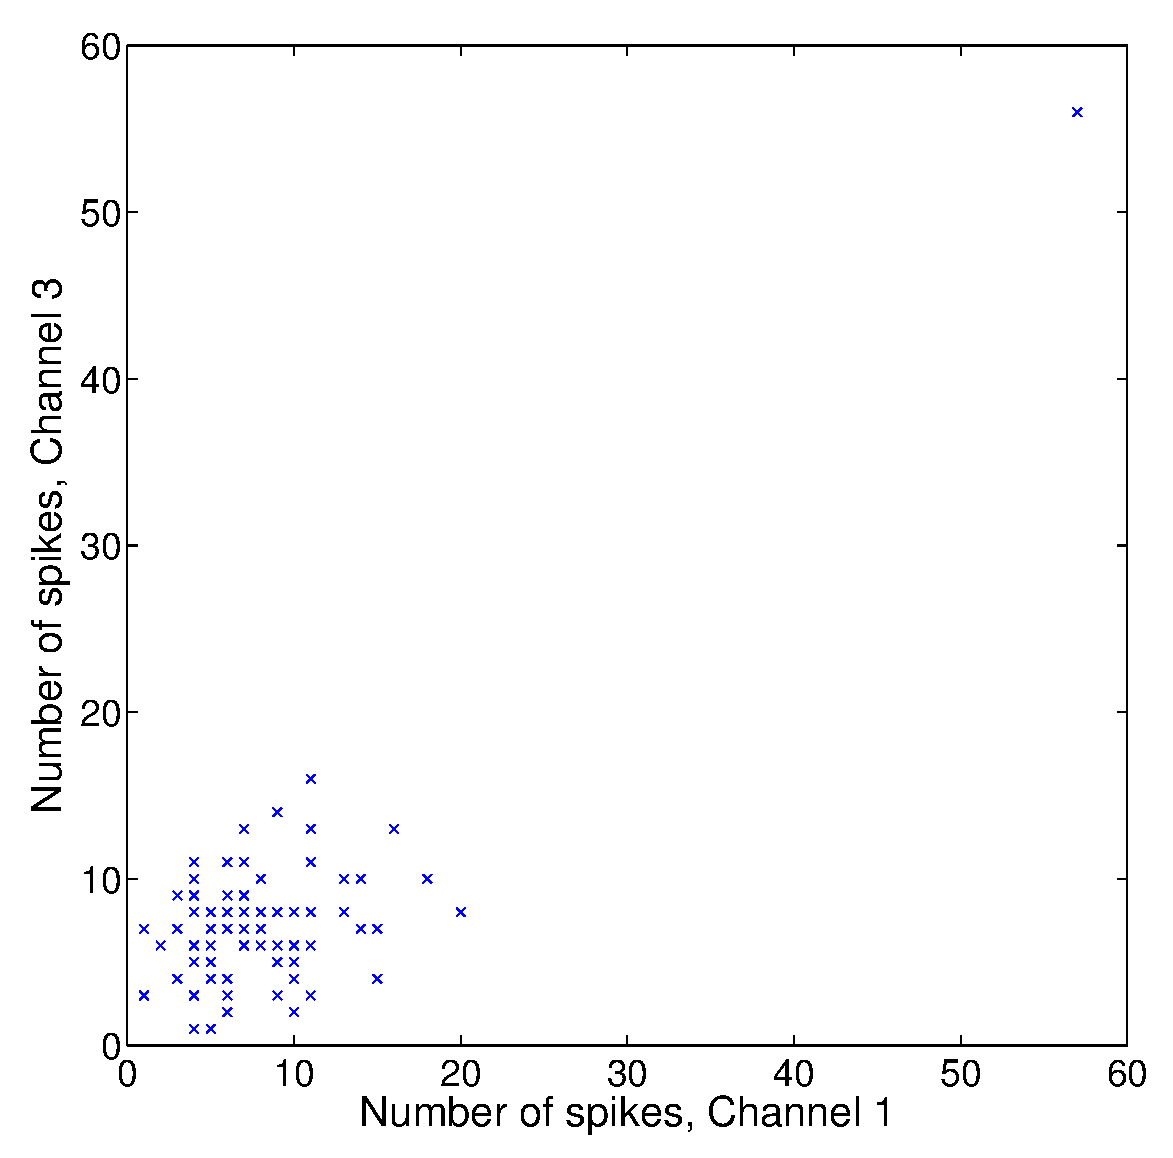
\includegraphics[width=0.4\linewidth]{%
figs/decoding/rcoef_scatter_jv4_icond5_ch1vch3.eps}
\caption{Spikes count during around \SI{500}{ms} of presentation of the \SI{27}{\percent} contrast stimulus, for two channels plotted against each other.
There is clearly a weak correlation between the two data-series, but one trial is an outlier with a large number of measured spikes for both channels due to a correlated source of noise in the raw signal.
The outlier will cause the correlation to be measured anomalously high.}
\label{fig:noise_scatter}
\end{figure}

To counter this problem, all trials where at least a quarter of the channels had a number of spikes more than 2.5 standard deviations above their mean spike count were removed.
This should be effective at fixing the problem because the motion-triggered artifact occurs always effects multiple channels simultaneously with the same artifact.
